\section{Additional Results on MPII Multi-Person}
Qualitative comparison of our joint formulation
$\deepcut~\multb~\dense$ to the traditional two-stage approach
$\dense~\detroi$ on MPII Multi-Person dataset is shown in
Fig.~\ref{fig:qualitative_mpii} and~\ref{fig:qualitative_mpii2}.
$\dense~\detroi$ works well when multiple fully visible individuals
are sufficiently separated and thus their body parts can be
partitioned based on the person detection bounding box. In this case
the strong $\dense$ body part detection model can correctly estimate
most of the visible body parts (image 16, 17, 19). However,
$\dense~\detroi$ cannot tell apart the body parts of multiple
individuals located next to each other and possibly occluding each
other, and often links the body parts across the individuals (images 1-16,
19-20). In addition, $\dense~\detroi$ cannot reason about occlusions
and truncations always providing a prediction for each body part
(image 4, 6, 10). In contrast, $\deepcut~\multb~\dense$ is able to
correctly partition and label an initial pool of body part candidates
(each image, top row) into subsets that correspond to sets of mutually
consistent body part candidates and abide to mutual consistency and
exclusion constraints (each image, row 2), thereby outputting
consistent body pose predictions (each image, row 3). $c \neq c'$
pairwise terms allow to partition the initial set of part detection
candidates into valid pose configurations (each image, row 2:
person-clusters highlighted by dense colored connections). $c = c'$
pairwise terms facilitate clustering of multiple body part candidates
of the same body part of the same person (each image, row 2: markers
of the same type and color). In addition, $c = c'$ pairwise terms
facilitate a repulsive property that prevents nearby part candidates
of the same type to be associated to different people (image 1:
detections of the left shoulder are assigned to the front person
only). Furthermore, $\deepcut~\multb~\dense$ allows to either merge
or deactivate part hypotheses thus effectively performing non-maximum
suppression and reasoning about body part occlusions and truncations
(image 3, row 2: body part hypotheses on the background are
deactivated (black crosses); image 6, row 2: body part hypotheses for
the truncated body parts are deactivated (black crosses); image 1-6,
8-9, 13-14, row 3: only visible body parts of the partially occluded
people are estimated, while non-visible body parts are correctly
predicted to be occluded). These qualitative examples show that
$\deepcuts~\multb$ can successfully deal with the unknown number of
people per image and the unknown number of visible body parts per
person.

\begin{figure*}
  \centering
  \begin{tabular}{c c c c c c c}
    &
%%     \includegraphics[height=0.140\linewidth]{imgidx_1346_init_graph_mpii_multi.pdf}&
    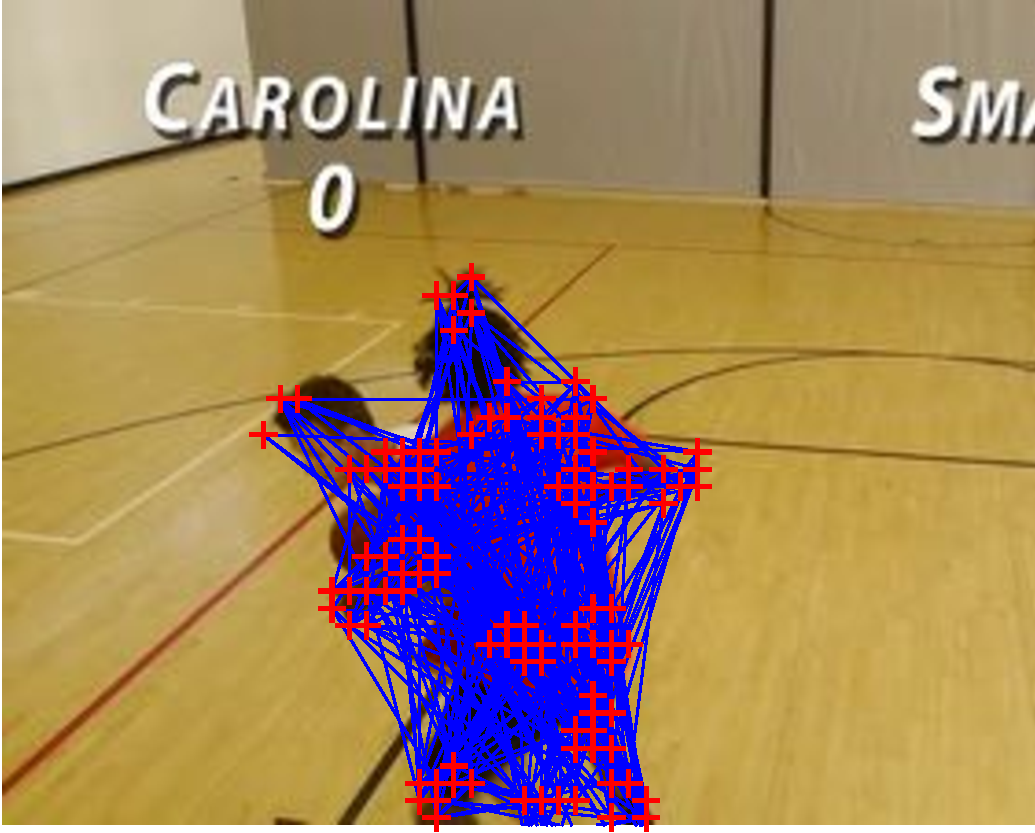
\includegraphics[height=0.140\linewidth]{imgidx_1674_init_graph_mpii_multi.pdf}&
    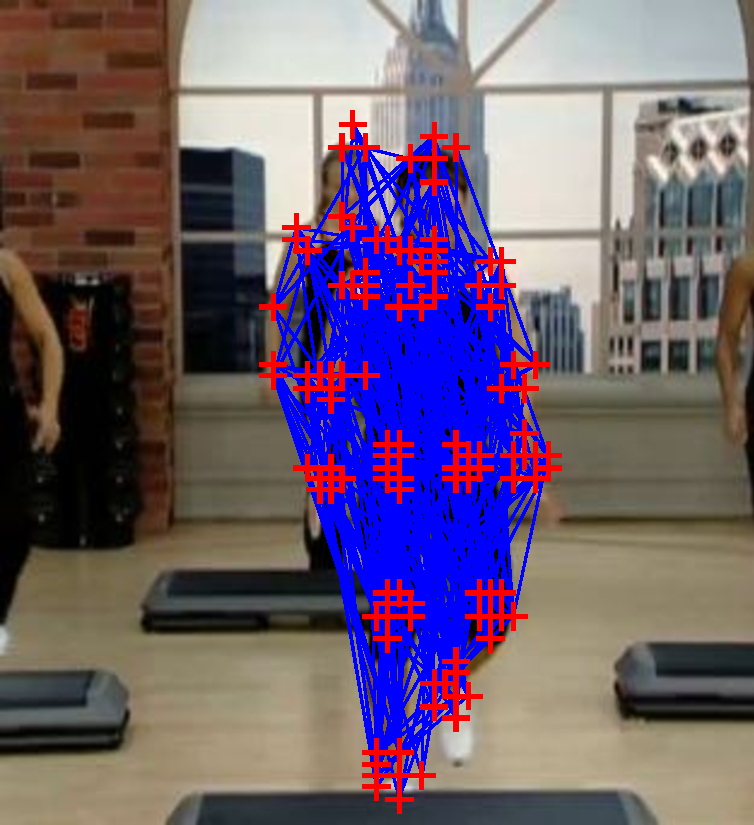
\includegraphics[height=0.140\linewidth]{imgidx_0564_init_graph_mpii_multi.pdf}&
%%     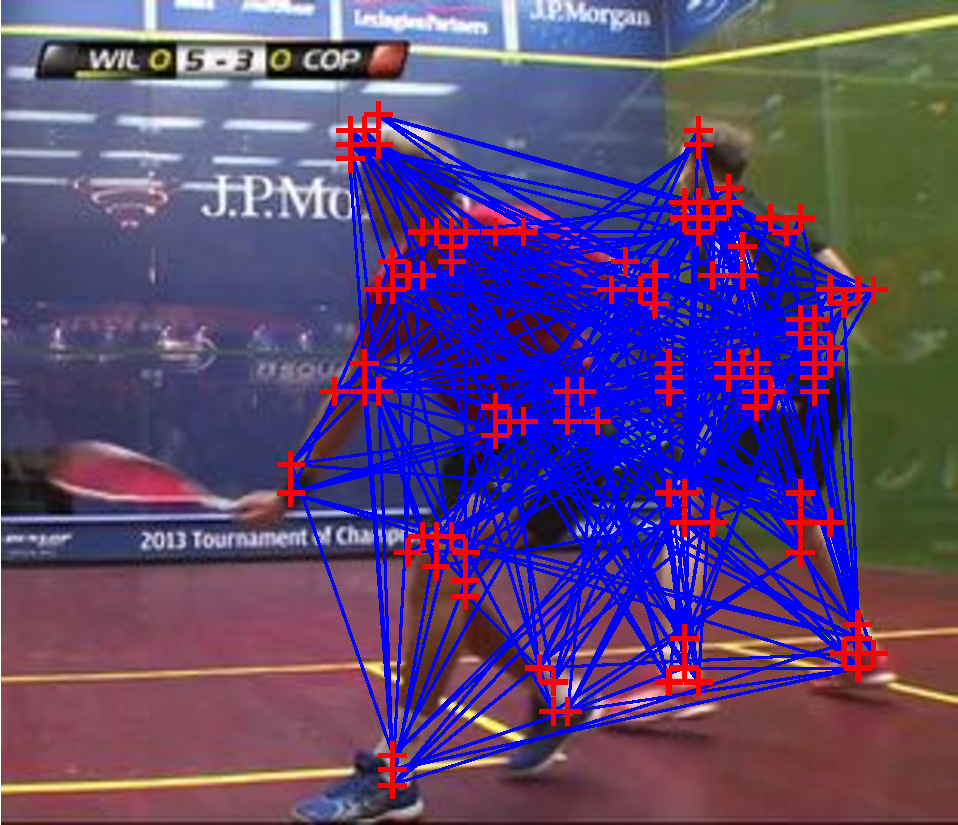
\includegraphics[height=0.140\linewidth]{imgidx_0908_init_graph_mpii_multi.pdf}&
%%     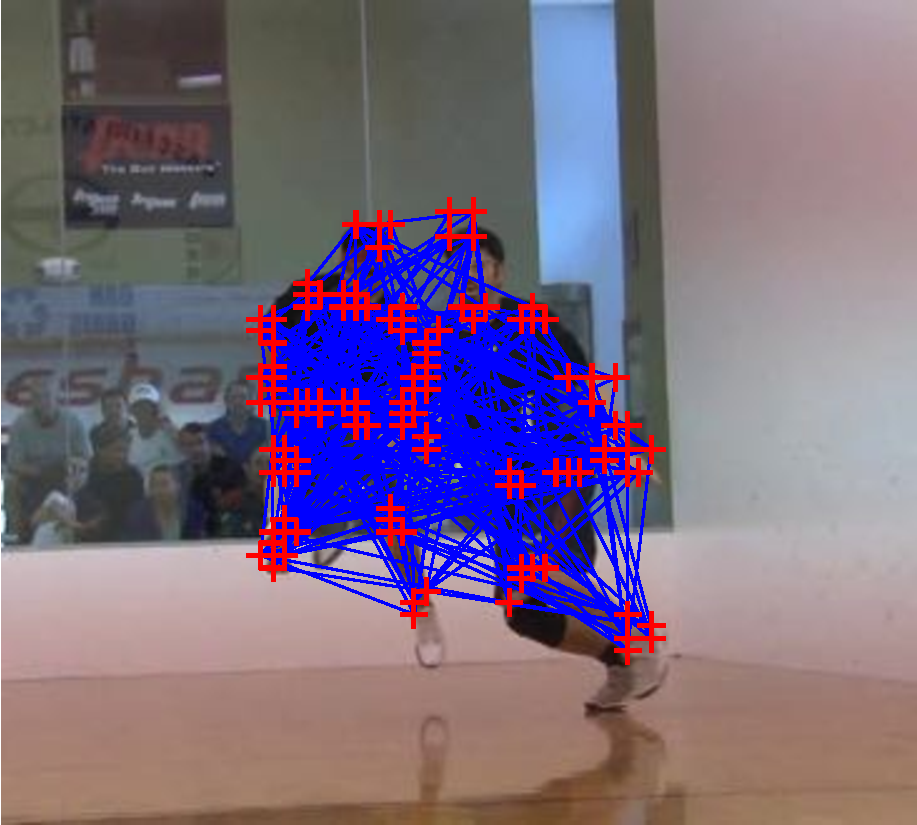
\includegraphics[height=0.140\linewidth]{imgidx_0104_init_graph_mpii_multi.pdf}&
    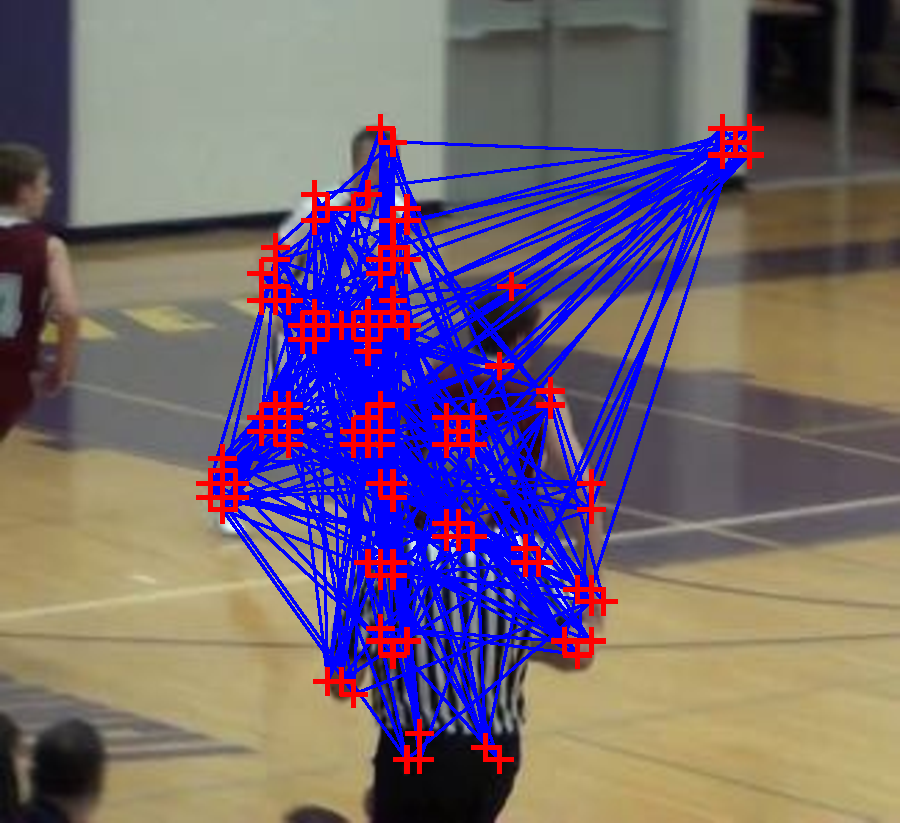
\includegraphics[height=0.140\linewidth]{imgidx_1652_init_graph_mpii_multi.pdf}&
    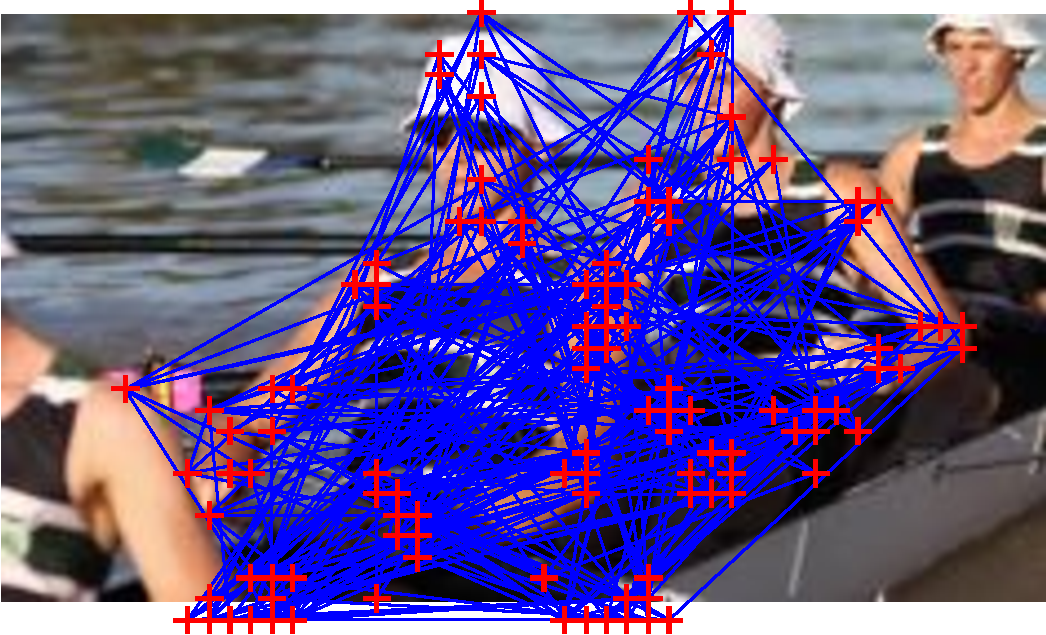
\includegraphics[height=0.140\linewidth]{imgidx_0472_init_graph_mpii_multi.pdf}&
    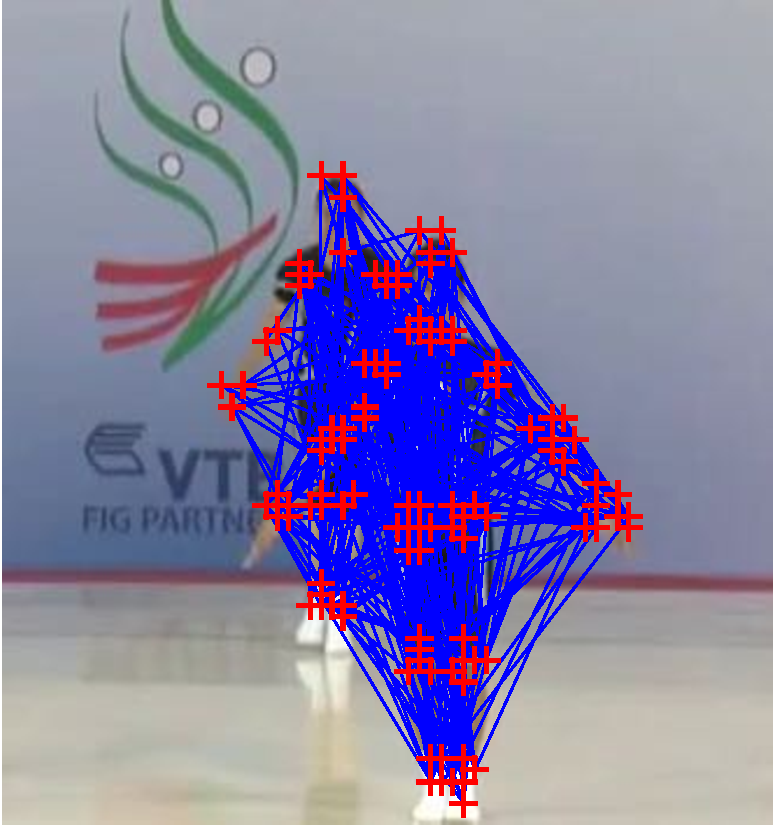
\includegraphics[height=0.140\linewidth]{imgidx_0630_init_graph_mpii_multi.pdf}\\
    \begin{sideways}\bf\quad $\deepcut~\multb$\end{sideways}&
%%     \includegraphics[height=0.140\linewidth]{imgidx_1346_graph_mpii_multi.pdf}&
    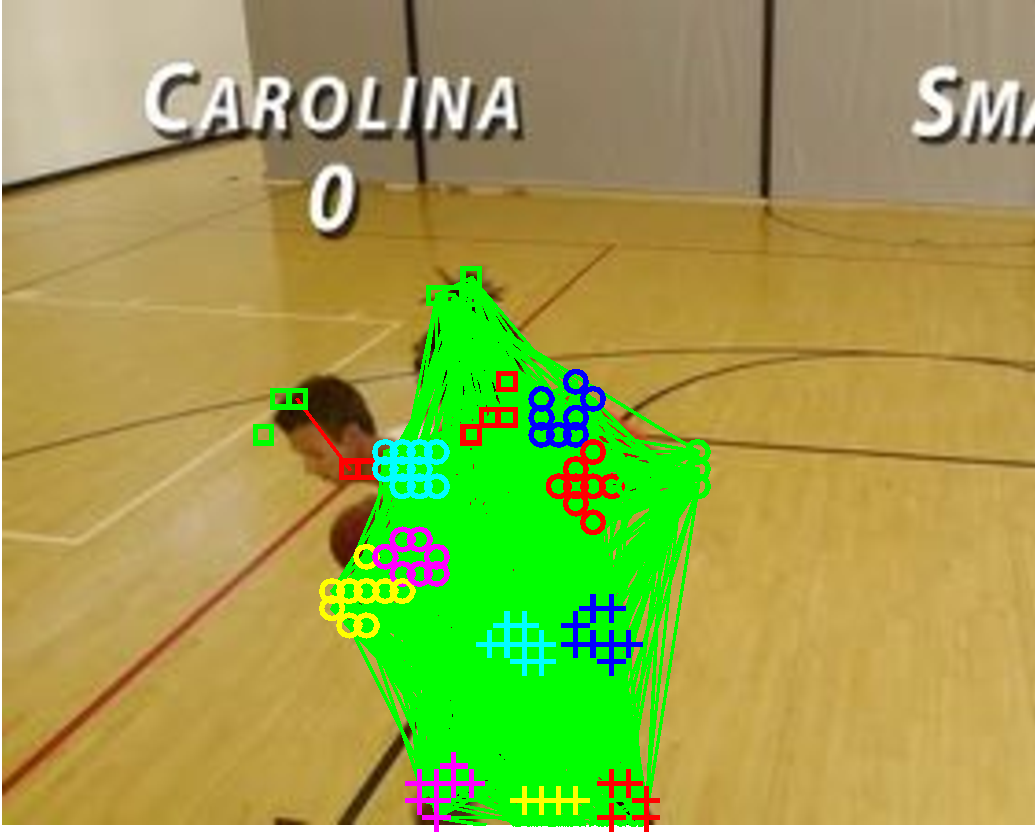
\includegraphics[height=0.140\linewidth]{imgidx_1674_graph_mpii_multi.pdf}&
    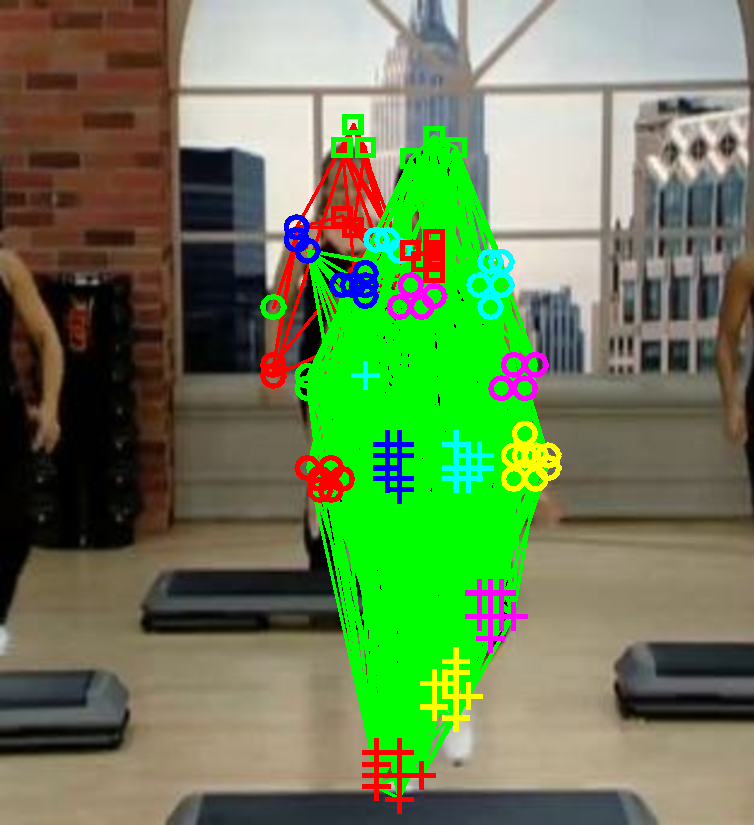
\includegraphics[height=0.140\linewidth]{imgidx_0564_graph_mpii_multi.pdf}&
%%     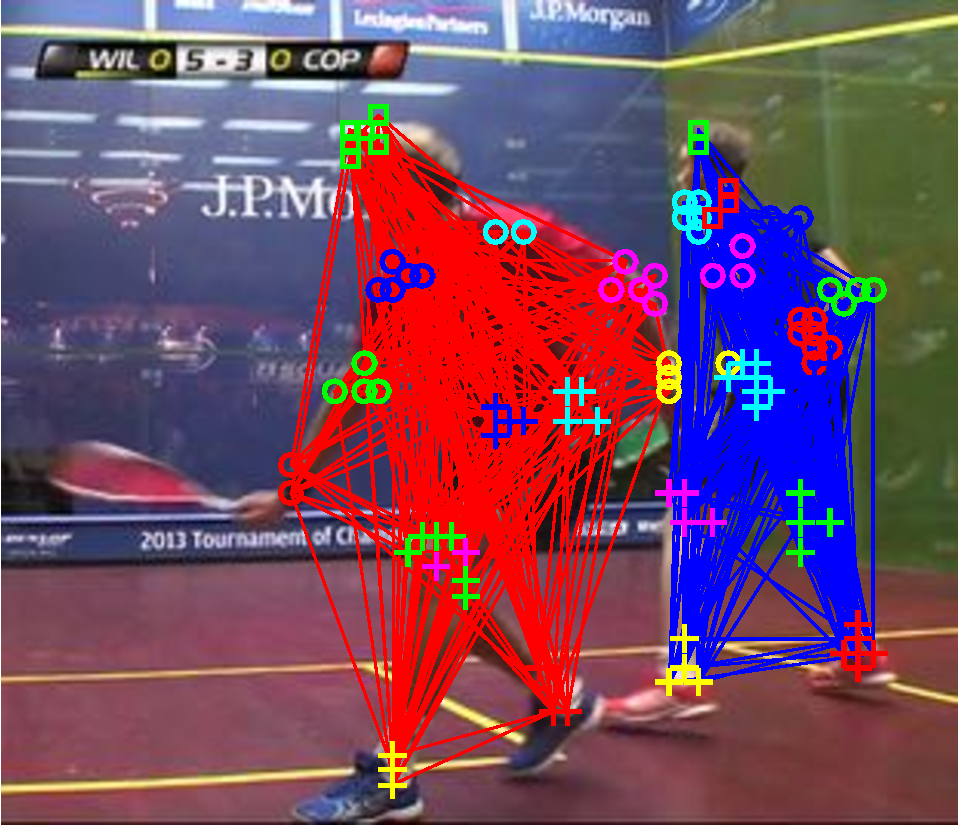
\includegraphics[height=0.140\linewidth]{imgidx_0908_graph_mpii_multi.pdf}&
%%     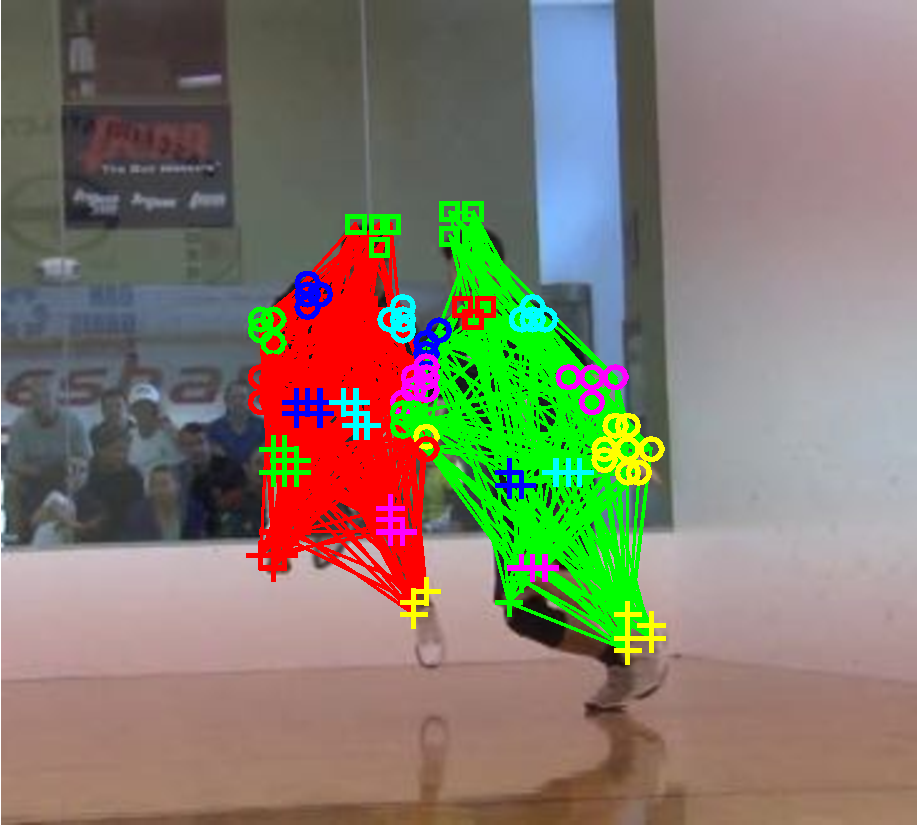
\includegraphics[height=0.140\linewidth]{imgidx_0104_graph_mpii_multi.pdf}&
    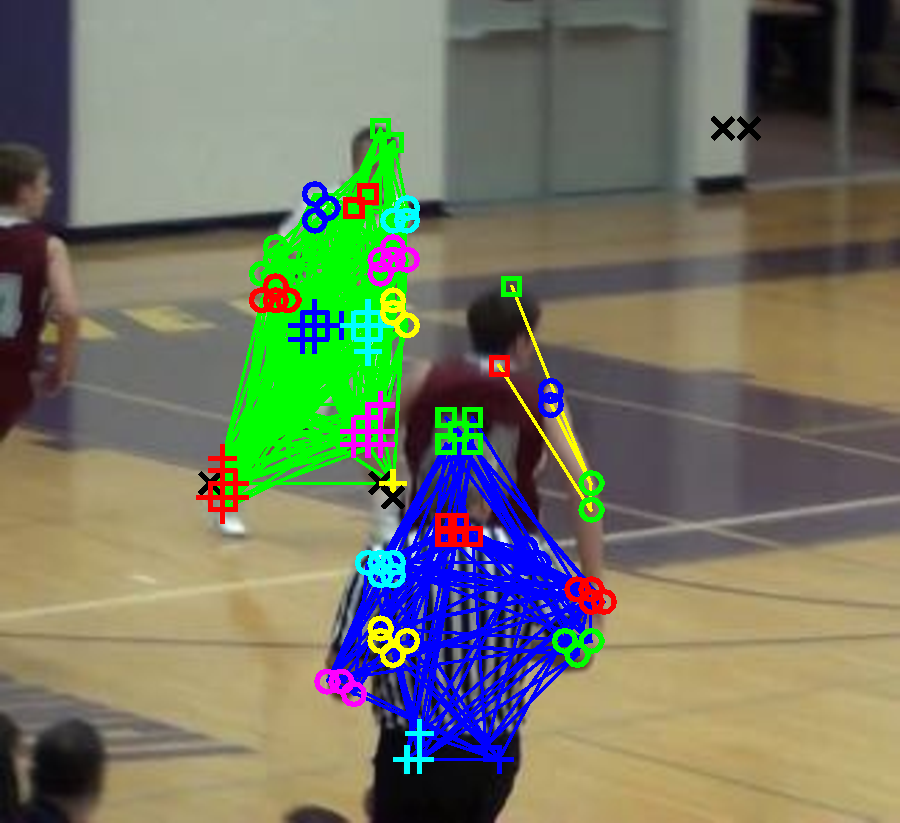
\includegraphics[height=0.140\linewidth]{imgidx_1652_graph_mpii_multi.pdf}&
    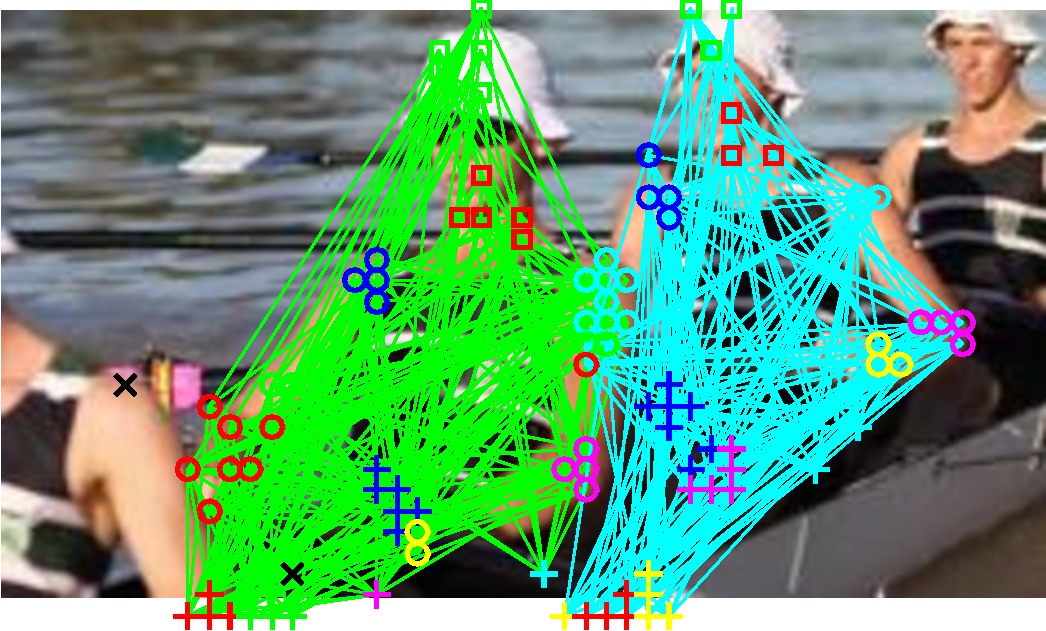
\includegraphics[height=0.140\linewidth]{imgidx_0472_graph_mpii_multi.pdf}&
    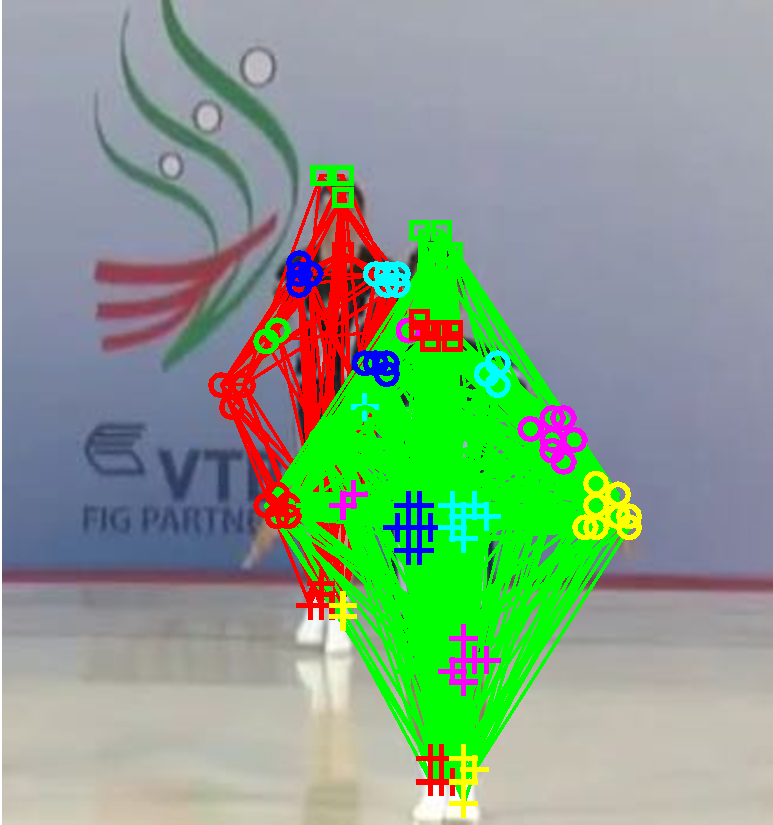
\includegraphics[height=0.140\linewidth]{imgidx_0630_graph_mpii_multi.pdf}\\
    &
%%     \includegraphics[height=0.140\linewidth]{imgidx_1346_sticks_mpii_multi.pdf}&
    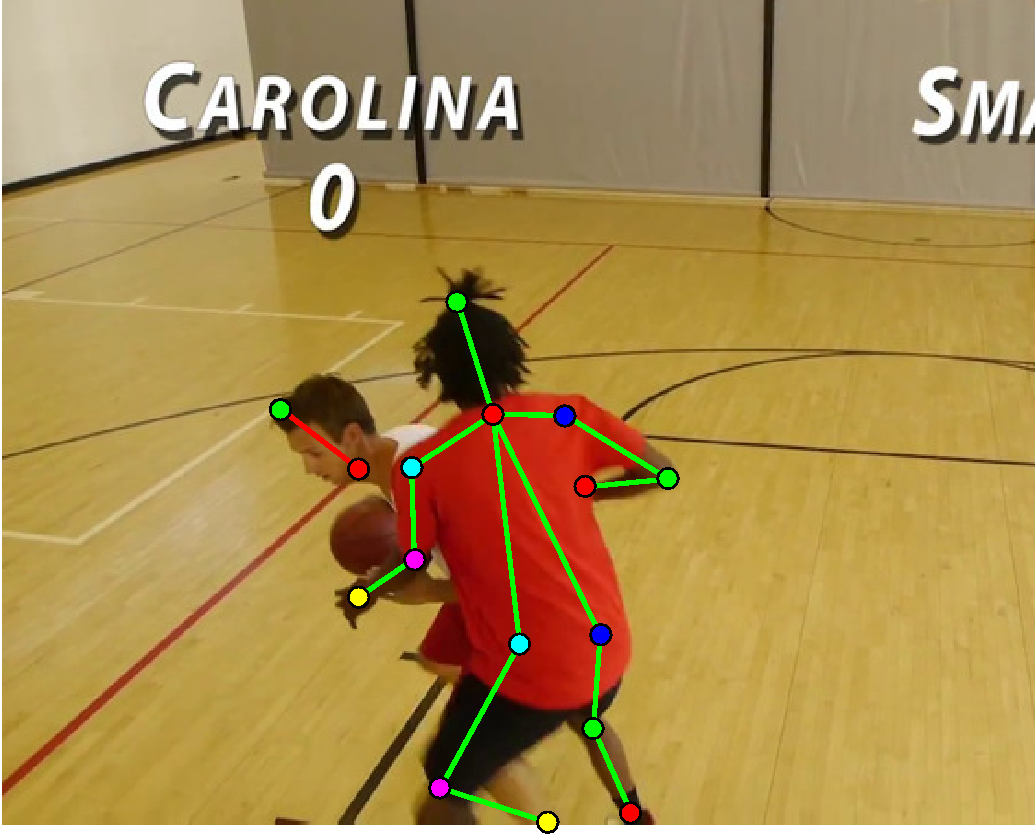
\includegraphics[height=0.140\linewidth]{imgidx_1674_sticks_mpii_multi.pdf}& 
    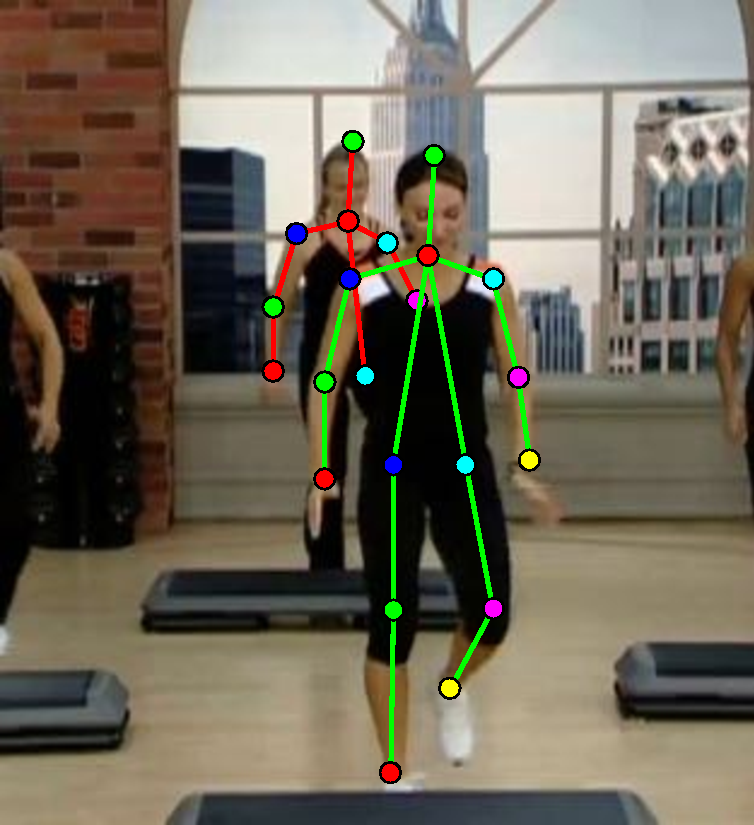
\includegraphics[height=0.140\linewidth]{imgidx_0564_sticks_mpii_multi.pdf}&
%%     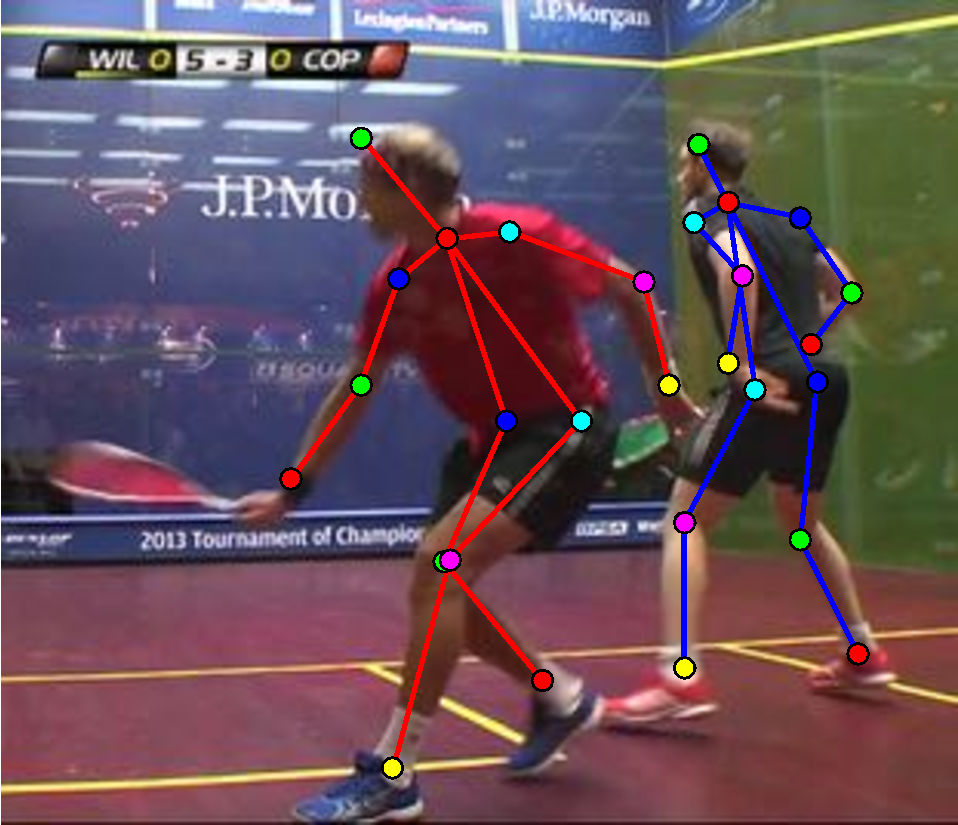
\includegraphics[height=0.140\linewidth]{imgidx_0908_sticks_mpii_multi.pdf}&
%%     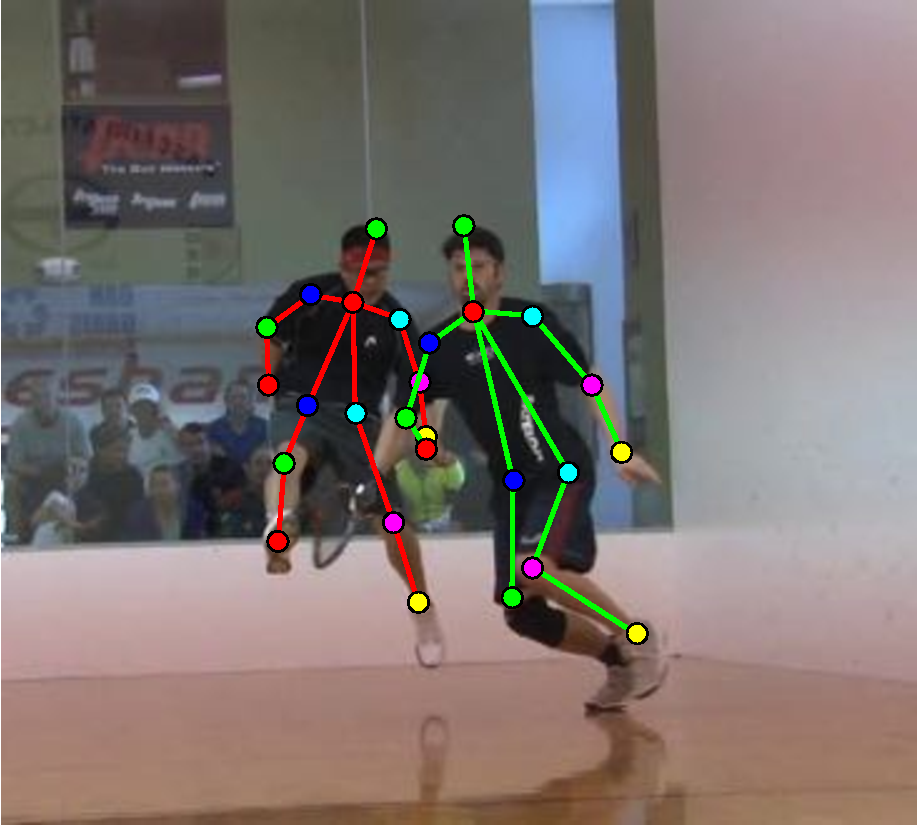
\includegraphics[height=0.140\linewidth]{imgidx_0104_sticks_mpii_multi.pdf}&
    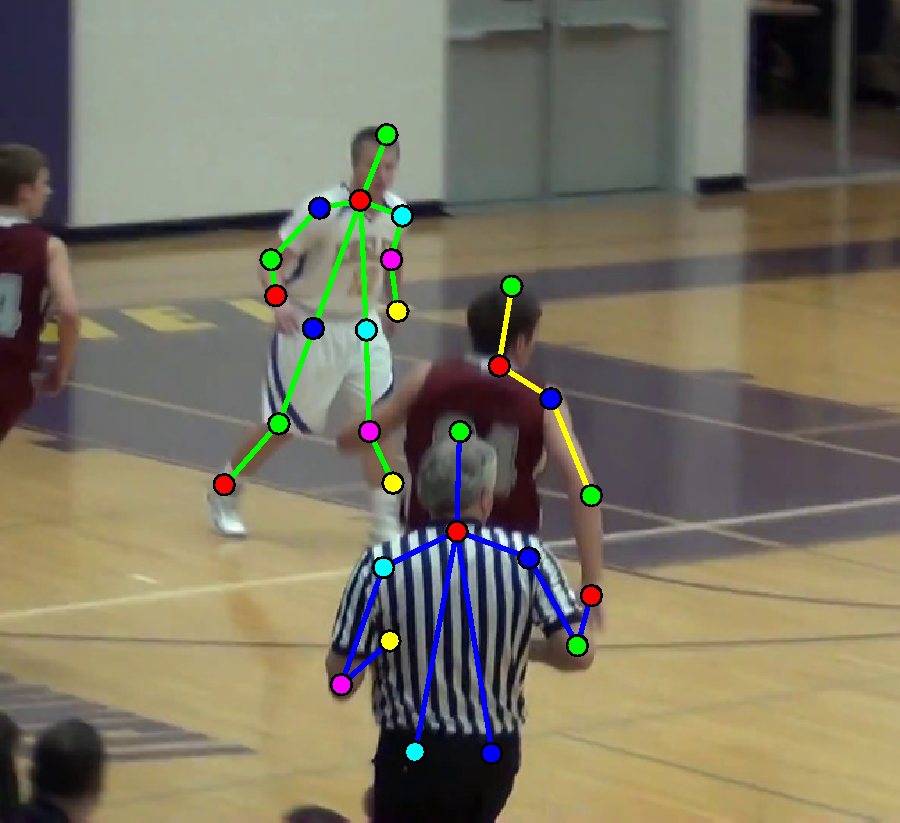
\includegraphics[height=0.140\linewidth]{imgidx_1652_sticks_mpii_multi.pdf}&
    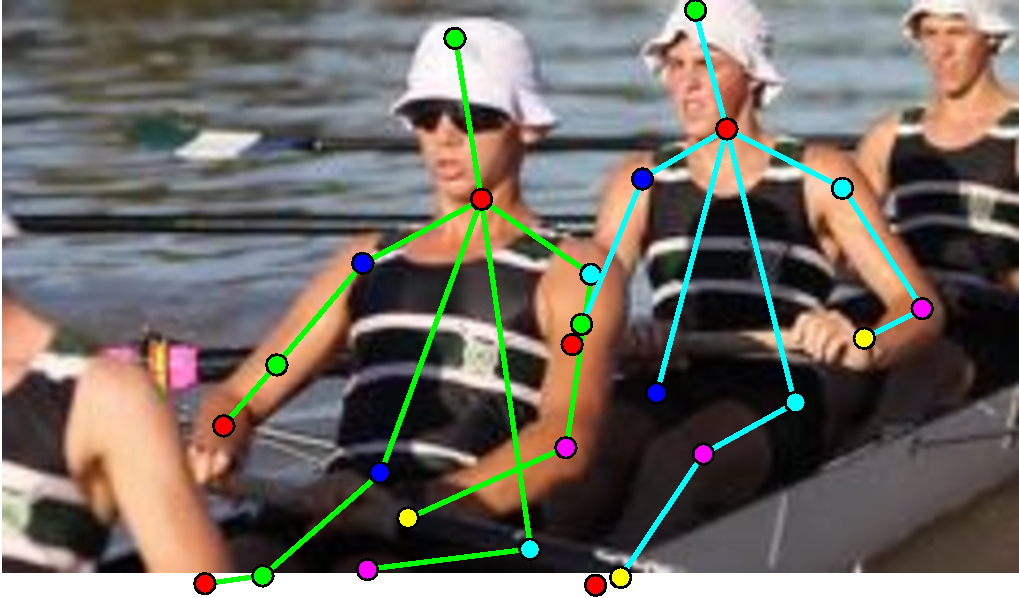
\includegraphics[height=0.140\linewidth]{imgidx_0472_sticks_mpii_multi.pdf}&
    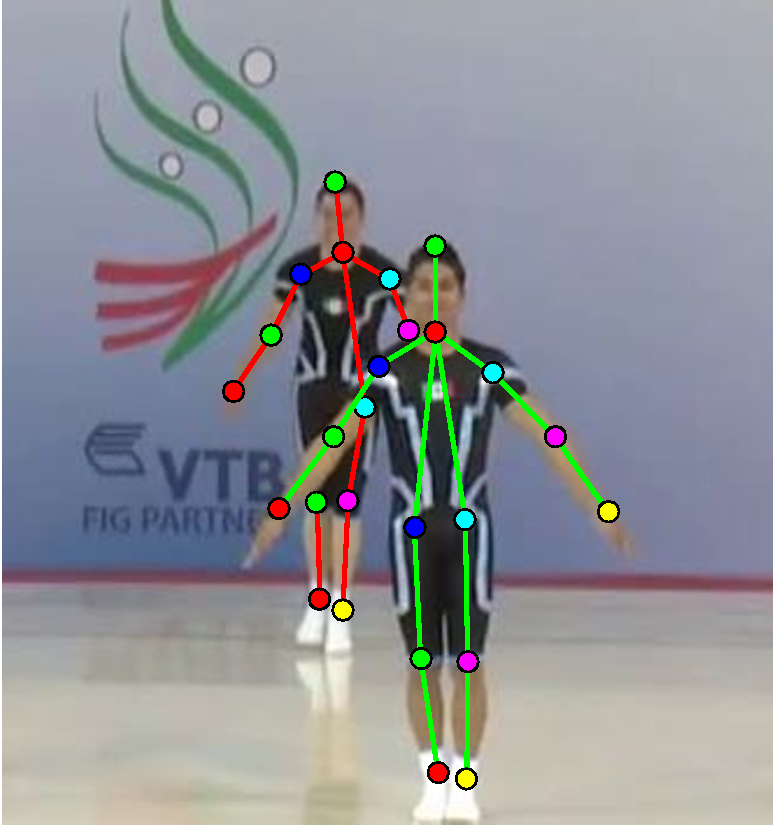
\includegraphics[height=0.140\linewidth]{imgidx_0630_sticks_mpii_multi.pdf}\\
    \midrule\midrule
    \begin{sideways}\bf \quad\quad$\detroi$\end{sideways}&
%%     \includegraphics[height=0.140\linewidth]{imgidx_1346_sticks_detroi_mpii_multi.pdf}&
    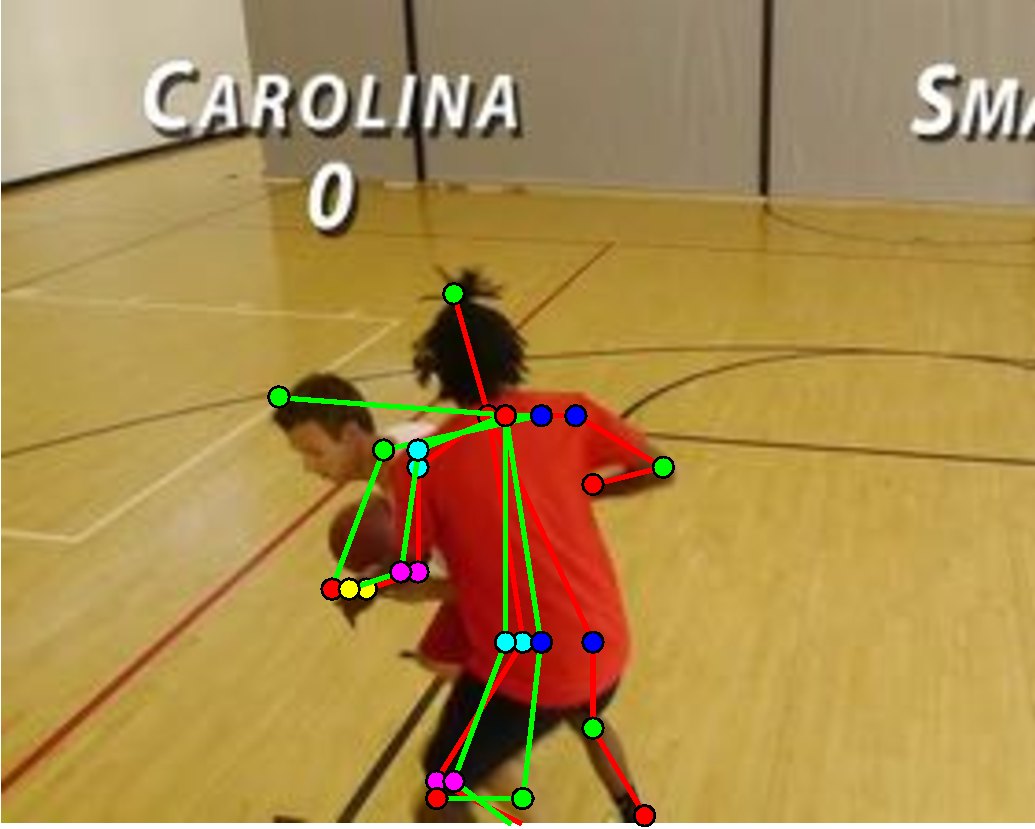
\includegraphics[height=0.140\linewidth]{imgidx_1674_sticks_detroi_mpii_multi.pdf}& 
    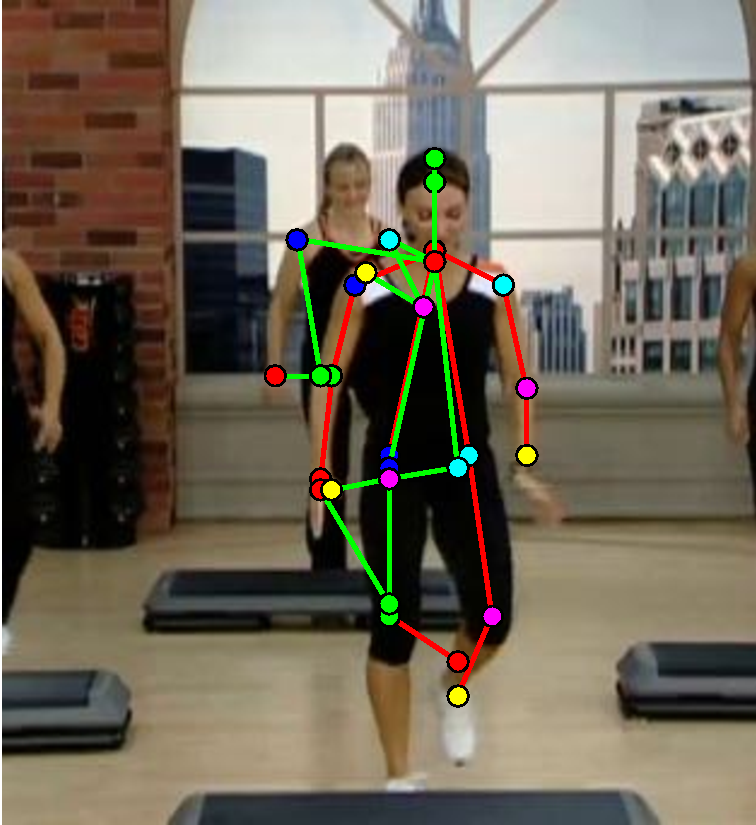
\includegraphics[height=0.140\linewidth]{imgidx_0564_sticks_detroi_mpii_multi.pdf}&
%%     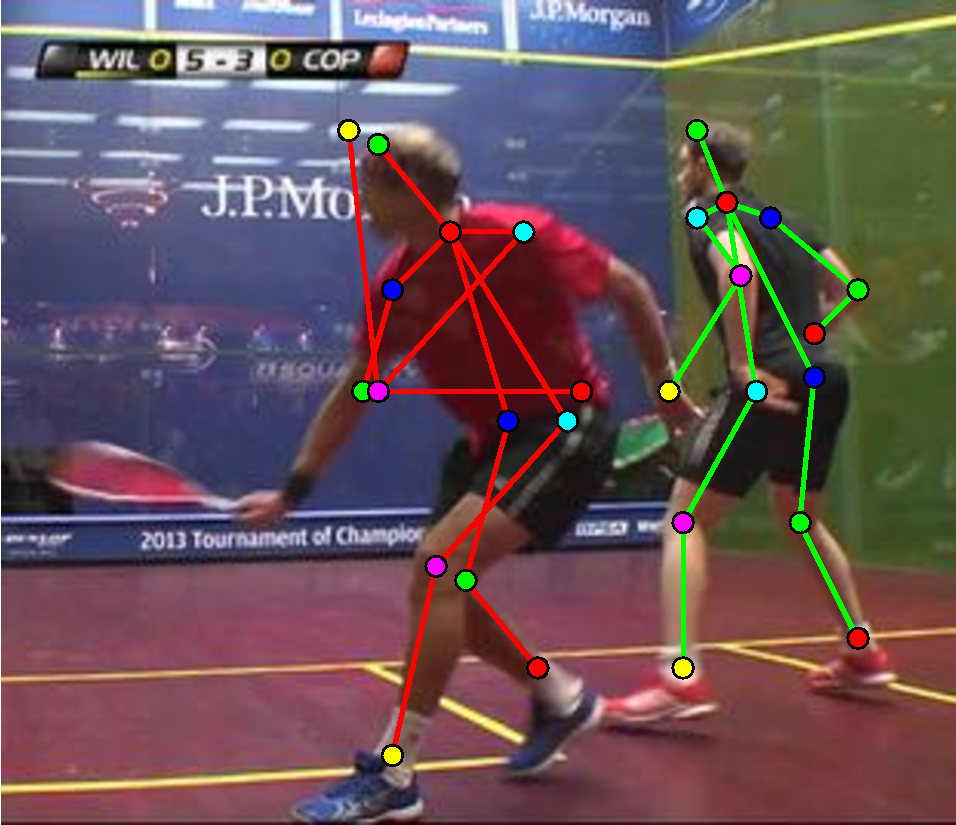
\includegraphics[height=0.140\linewidth]{imgidx_0908_sticks_detroi_mpii_multi.pdf}&
%%     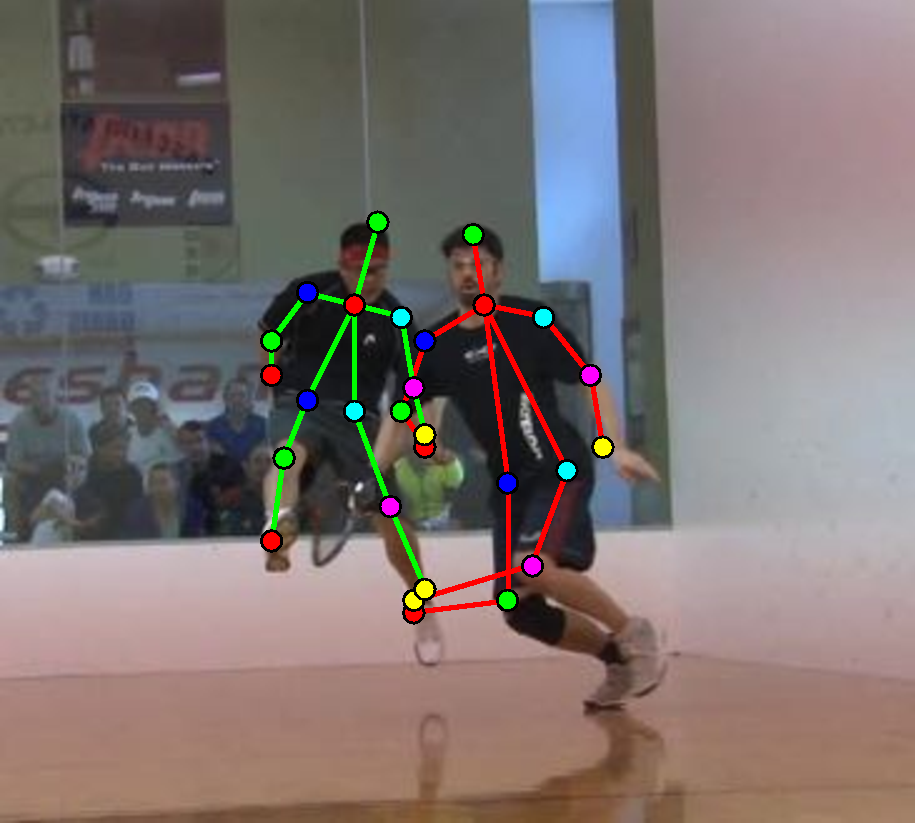
\includegraphics[height=0.140\linewidth]{imgidx_0104_sticks_detroi_mpii_multi.pdf}&
    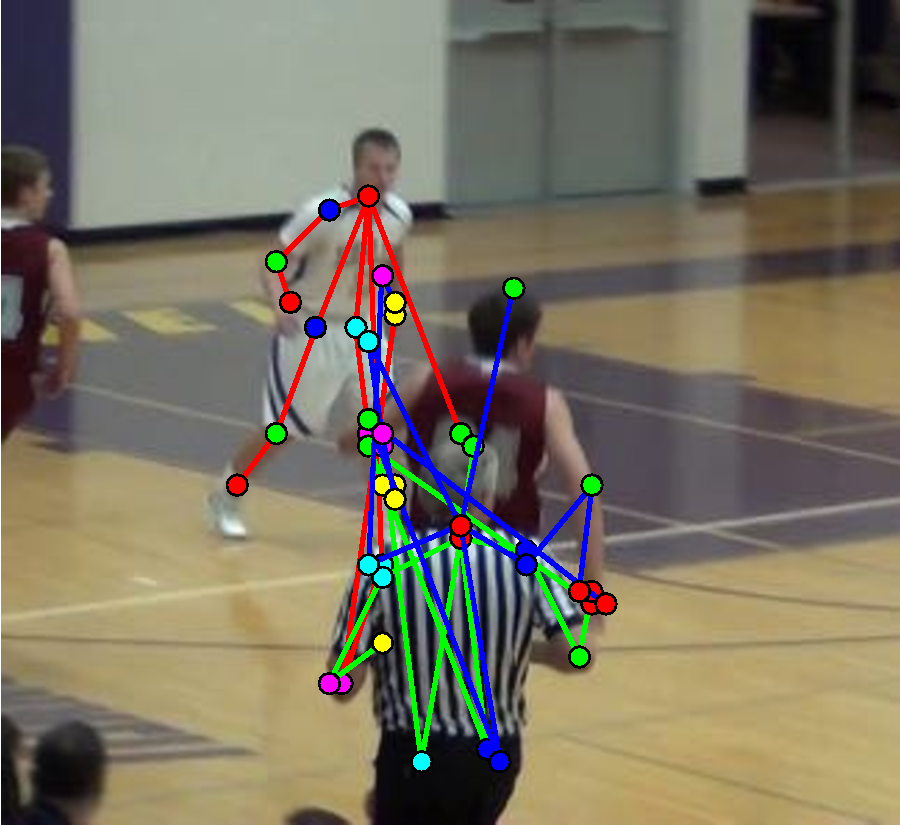
\includegraphics[height=0.140\linewidth]{imgidx_1652_sticks_detroi_mpii_multi.pdf}&
    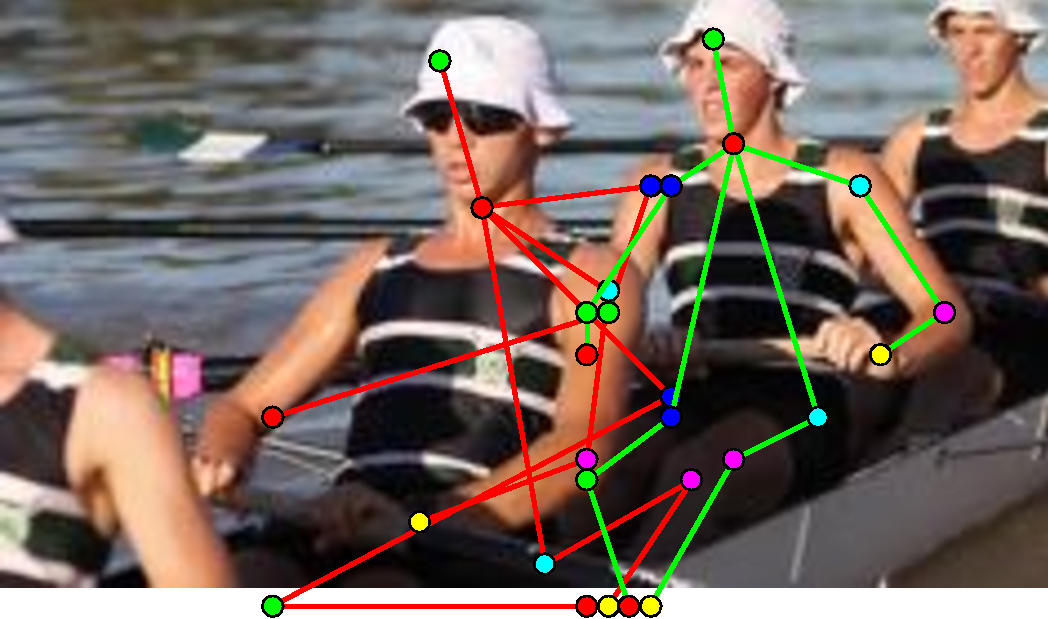
\includegraphics[height=0.140\linewidth]{imgidx_0472_sticks_detroi_mpii_multi.pdf}&
    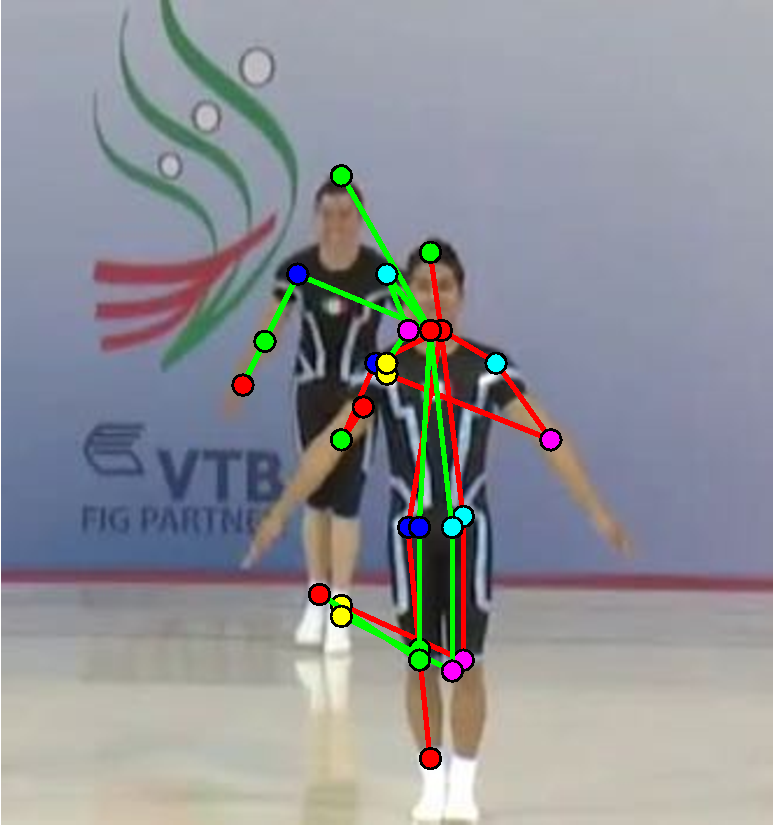
\includegraphics[height=0.140\linewidth]{imgidx_0630_sticks_detroi_mpii_multi.pdf}\\
    %&&&&\\
  &1&2&3&4&5\\  
  \end{tabular}

  \begin{tabular}{c c c c c c c}
    \toprule
    &
    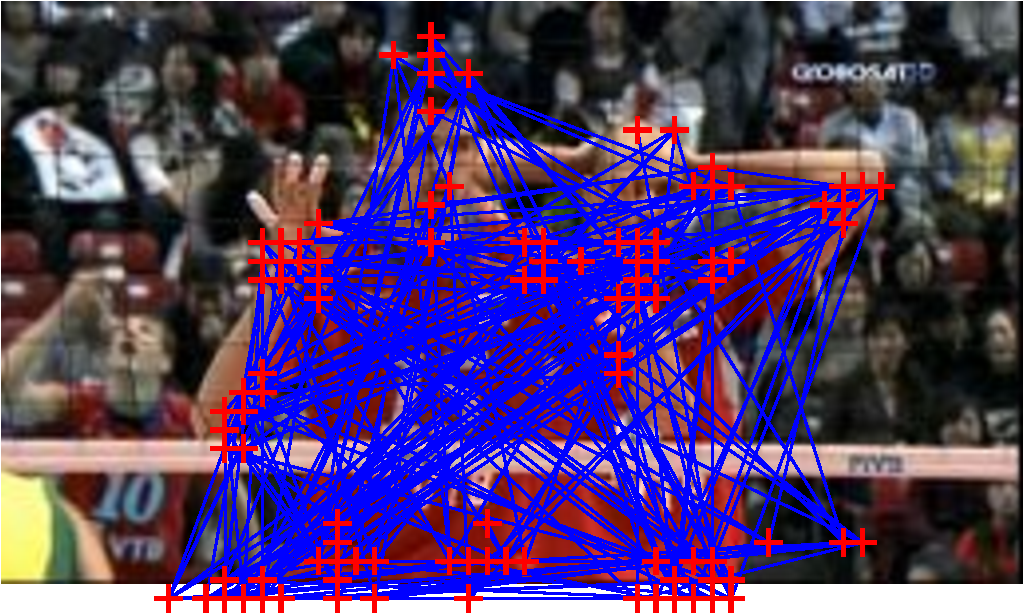
\includegraphics[height=0.140\linewidth]{imgidx_0092_init_graph_mpii_multi.pdf}&
    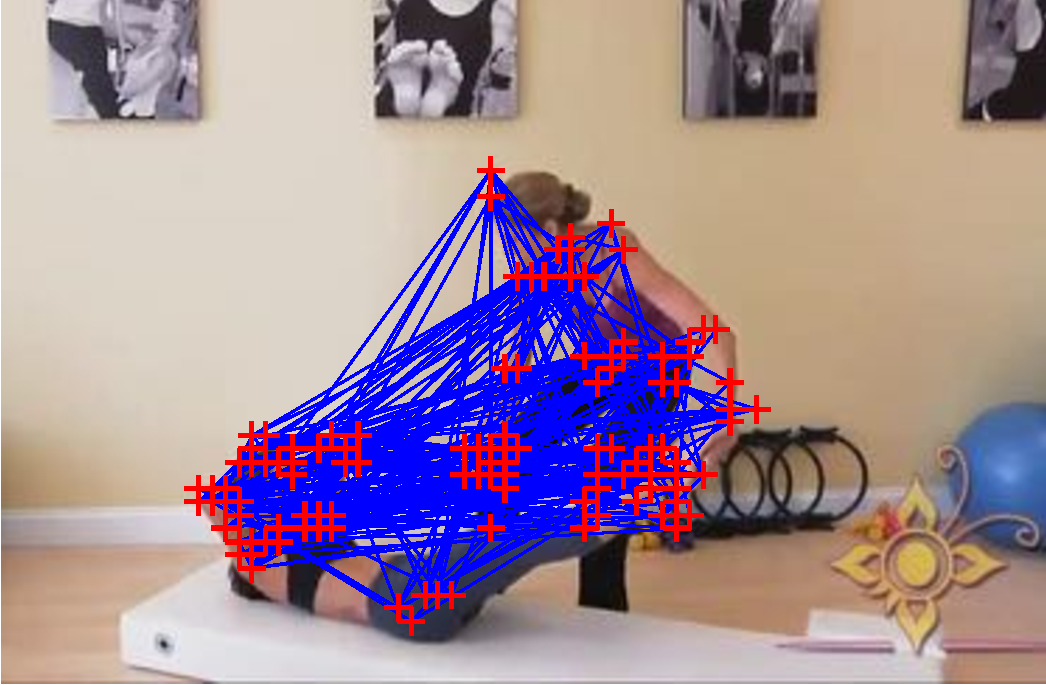
\includegraphics[height=0.140\linewidth]{imgidx_1366_init_graph_mpii_multi.pdf}&
%%     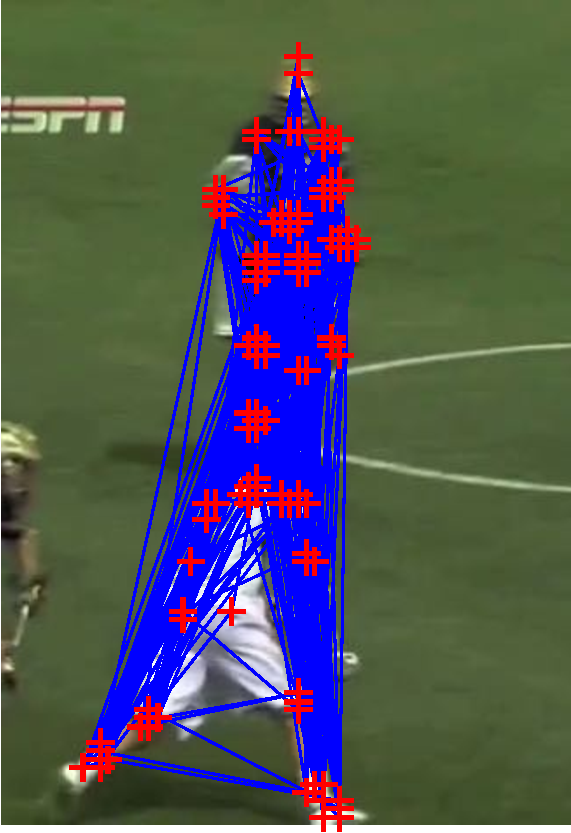
\includegraphics[height=0.140\linewidth]{imgidx_1589_init_graph_mpii_multi.pdf}&
%%     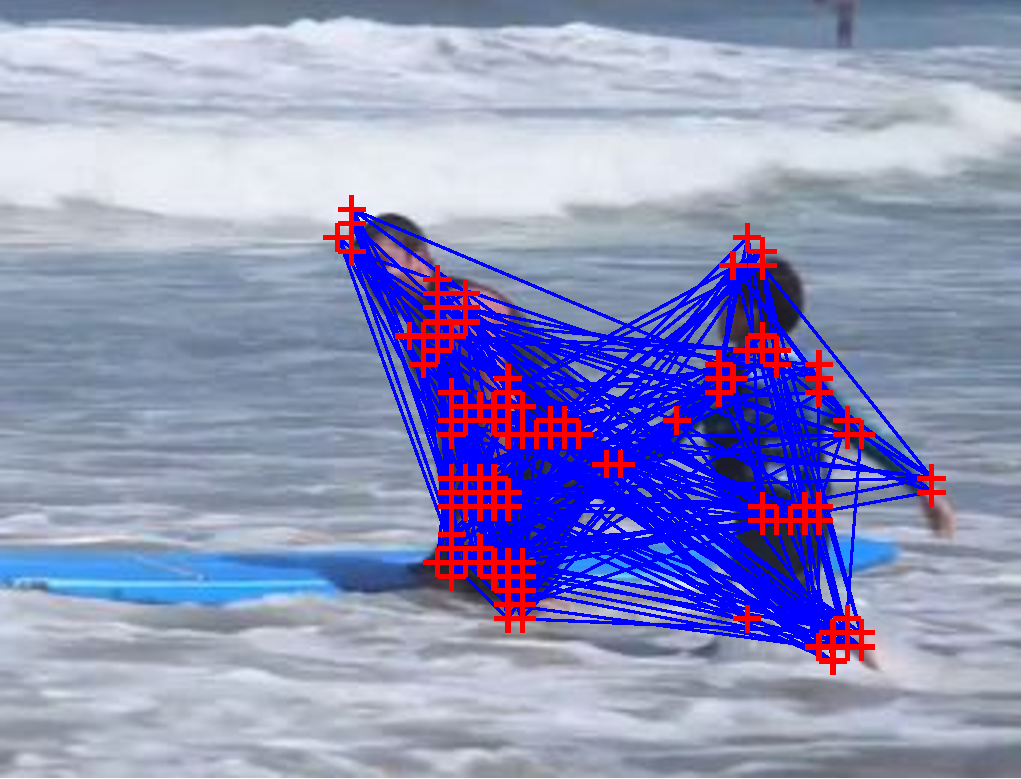
\includegraphics[height=0.140\linewidth]{imgidx_1183_init_graph_mpii_multi.pdf}&
    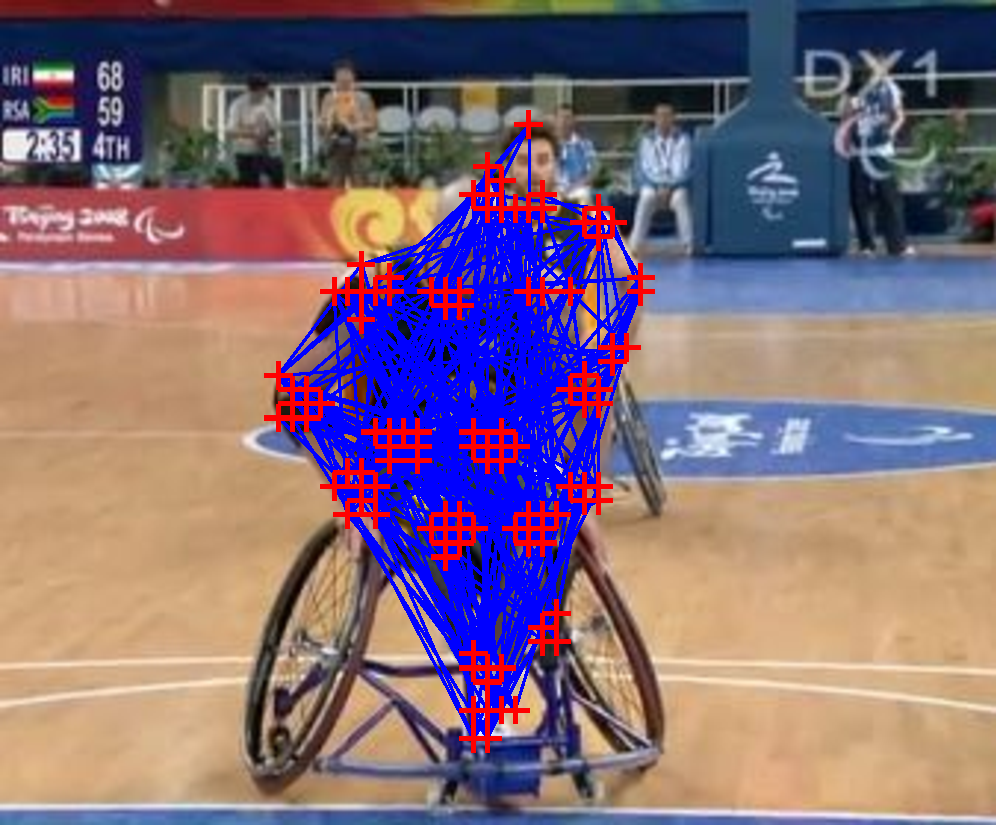
\includegraphics[height=0.140\linewidth]{imgidx_0094_init_graph_mpii_multi.pdf}&
    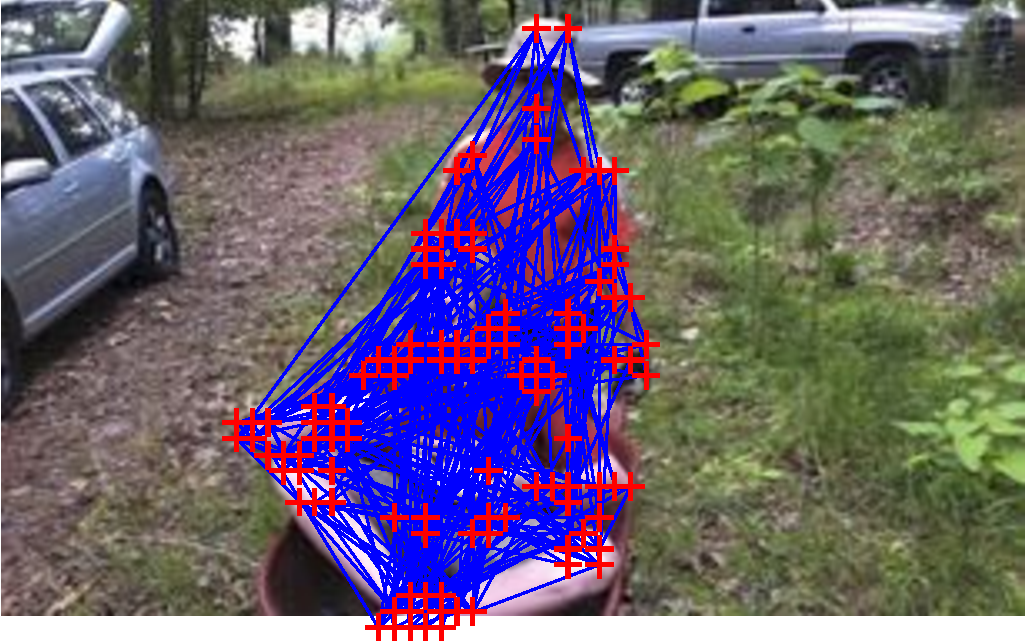
\includegraphics[height=0.140\linewidth]{imgidx_0903_init_graph_mpii_multi.pdf}\\
    \begin{sideways}\bf\quad $\deepcut~\multb$\end{sideways}&    
    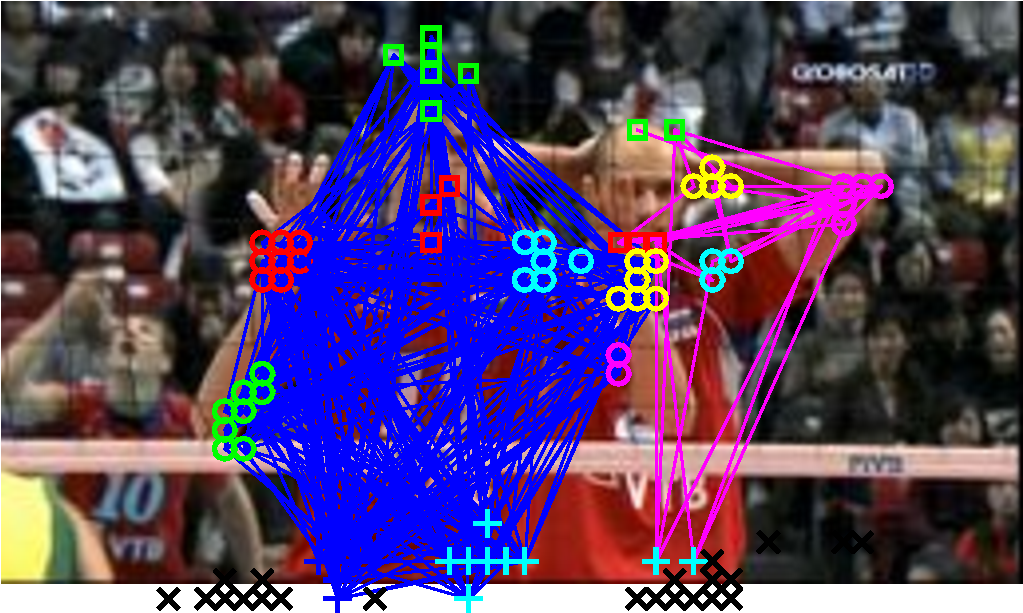
\includegraphics[height=0.140\linewidth]{imgidx_0092_graph_mpii_multi.pdf}&
    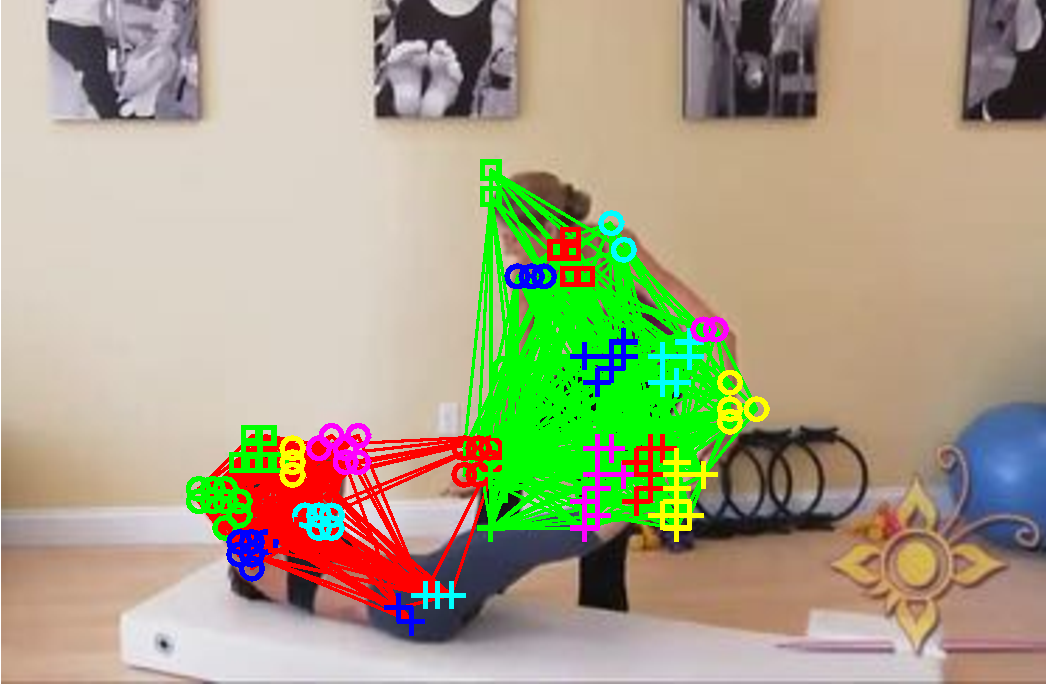
\includegraphics[height=0.140\linewidth]{imgidx_1366_graph_mpii_multi.pdf}&
%%     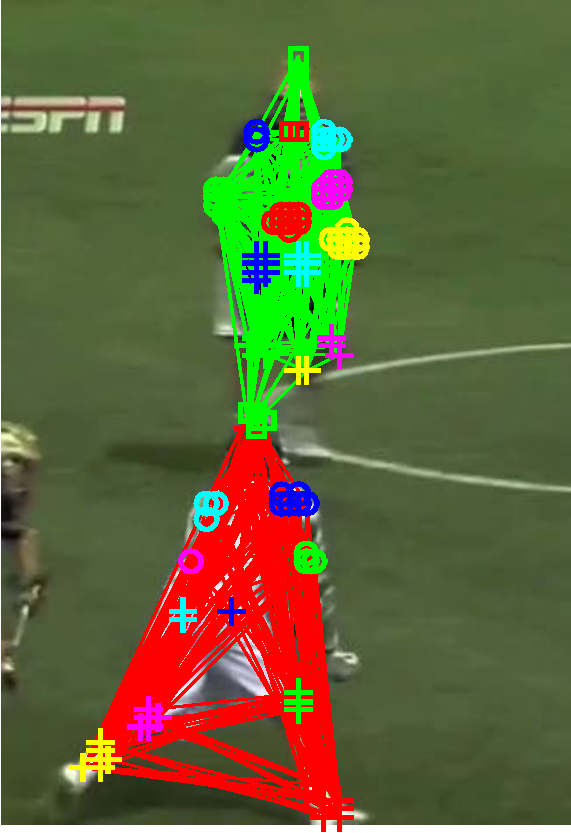
\includegraphics[height=0.140\linewidth]{imgidx_1589_graph_mpii_multi.pdf}&
%%     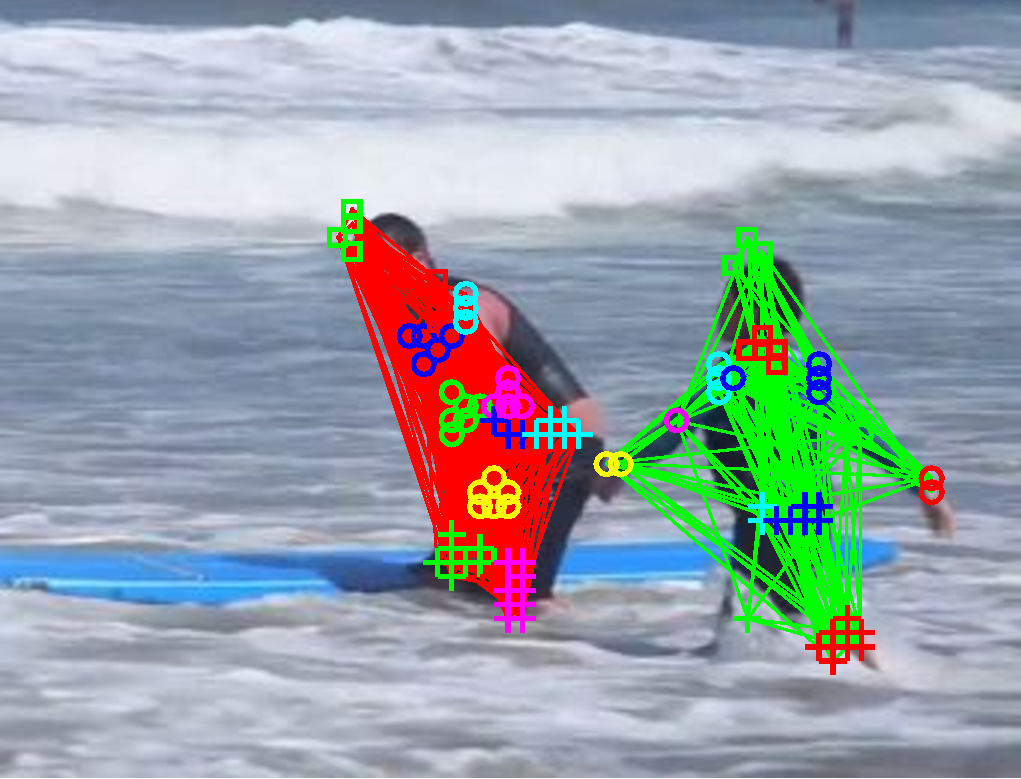
\includegraphics[height=0.140\linewidth]{imgidx_1183_graph_mpii_multi.pdf}&
    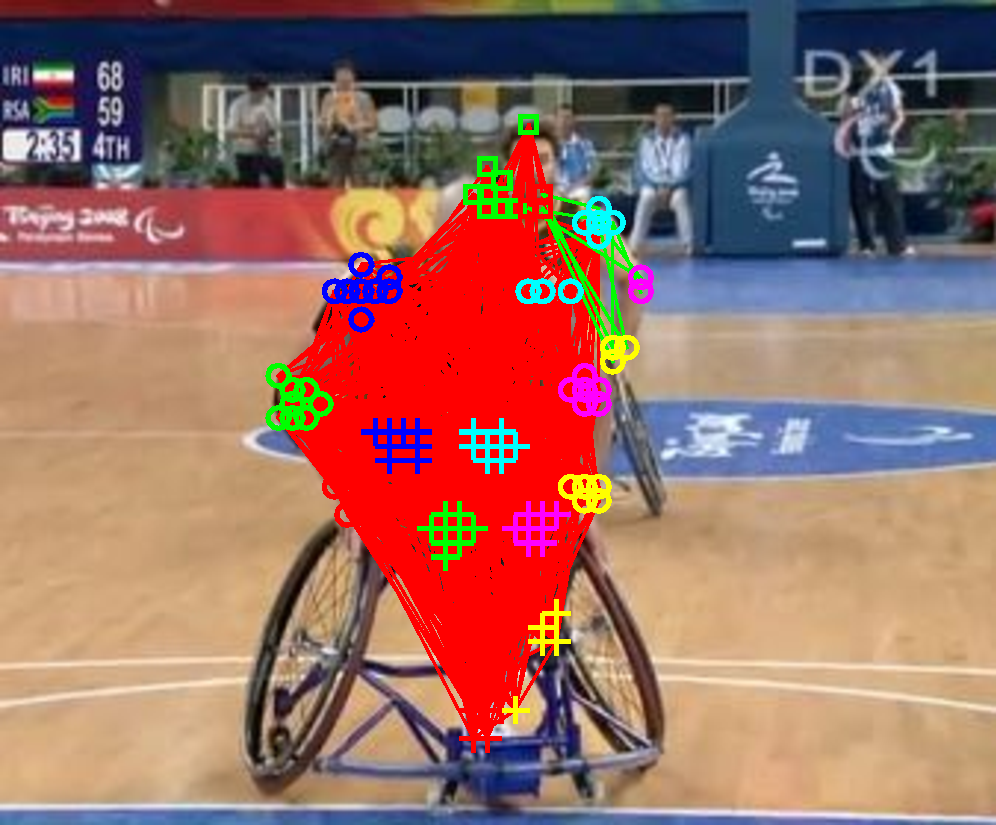
\includegraphics[height=0.140\linewidth]{imgidx_0094_graph_mpii_multi.pdf}&
    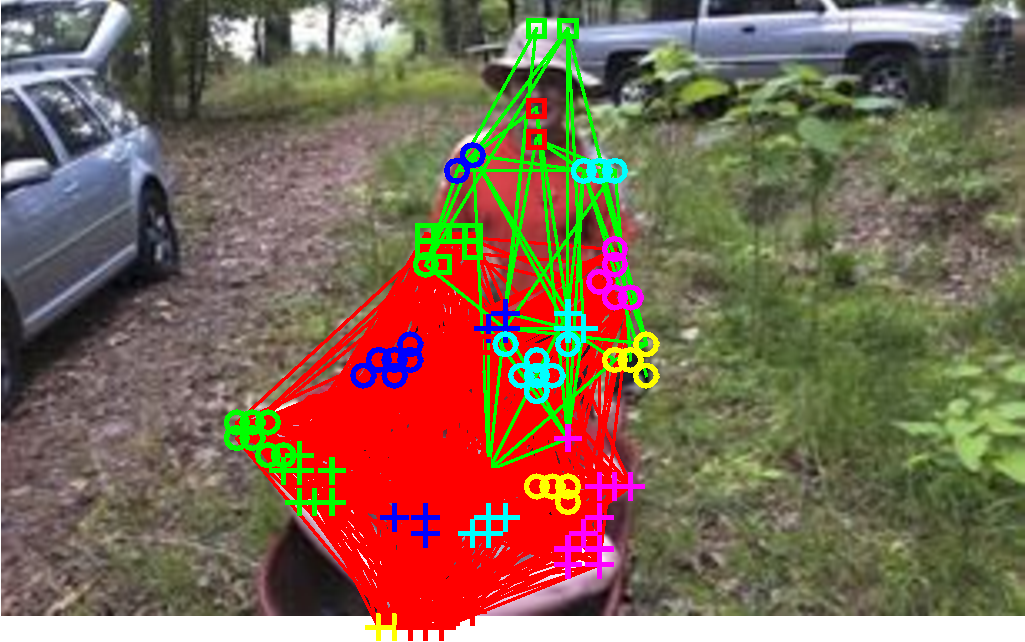
\includegraphics[height=0.140\linewidth]{imgidx_0903_graph_mpii_multi.pdf}\\
    &
    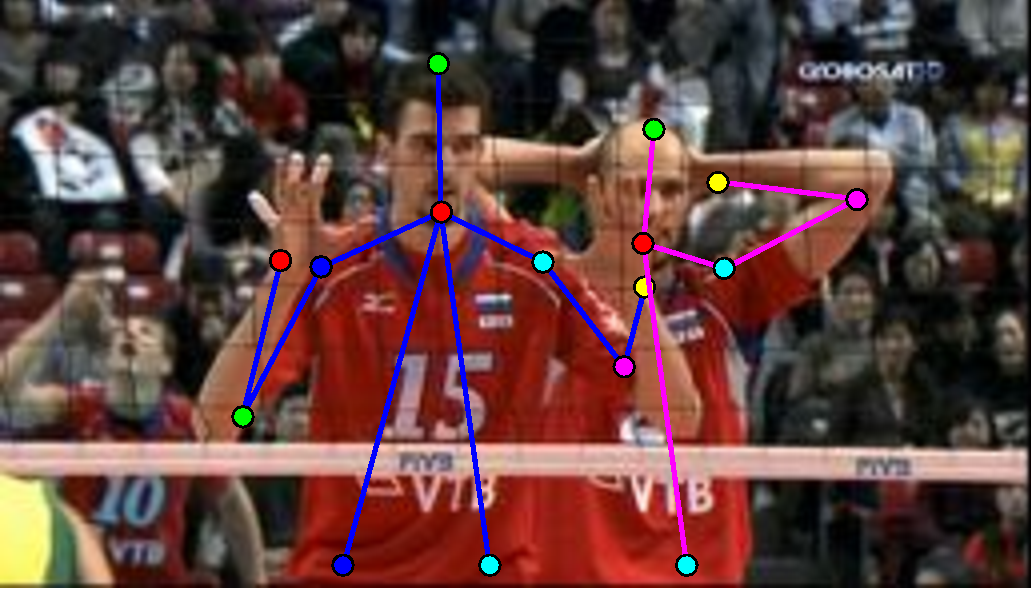
\includegraphics[height=0.140\linewidth]{imgidx_0092_sticks_mpii_multi.pdf}&
    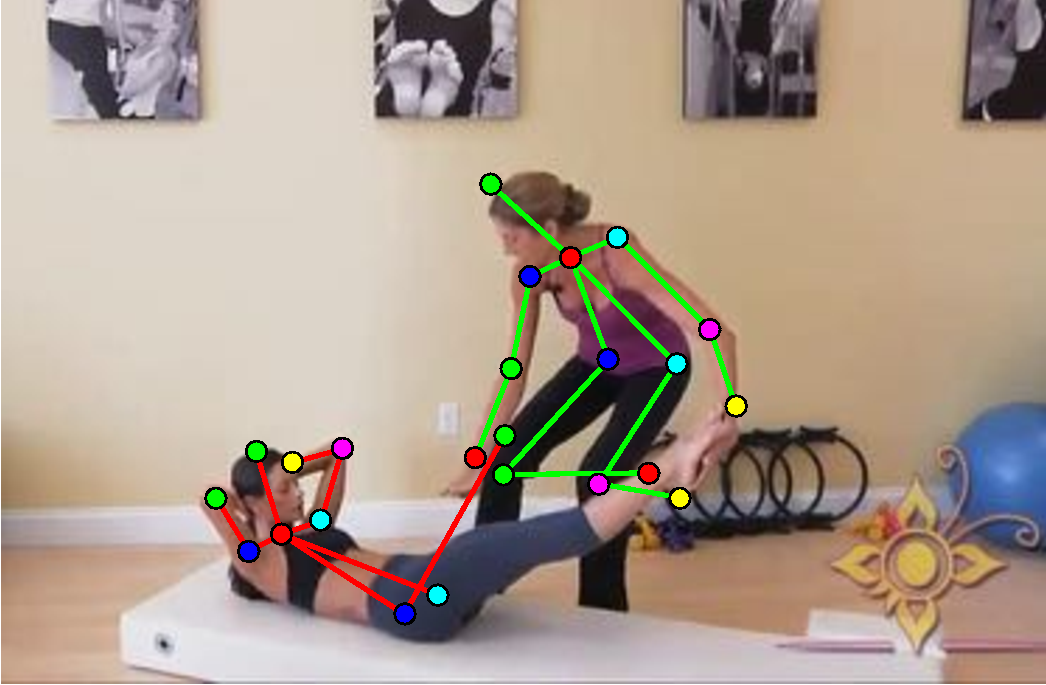
\includegraphics[height=0.140\linewidth]{imgidx_1366_sticks_mpii_multi.pdf}& 
%%     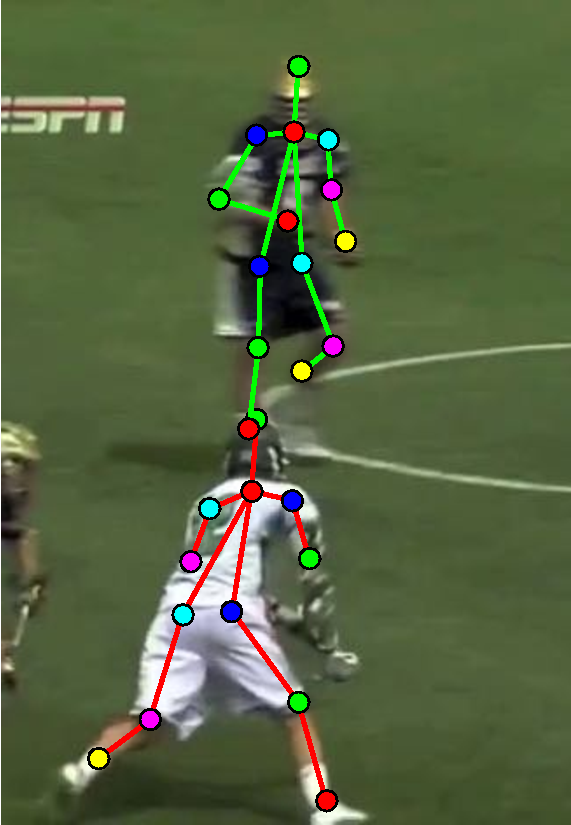
\includegraphics[height=0.140\linewidth]{imgidx_1589_sticks_mpii_multi.pdf}&
%%     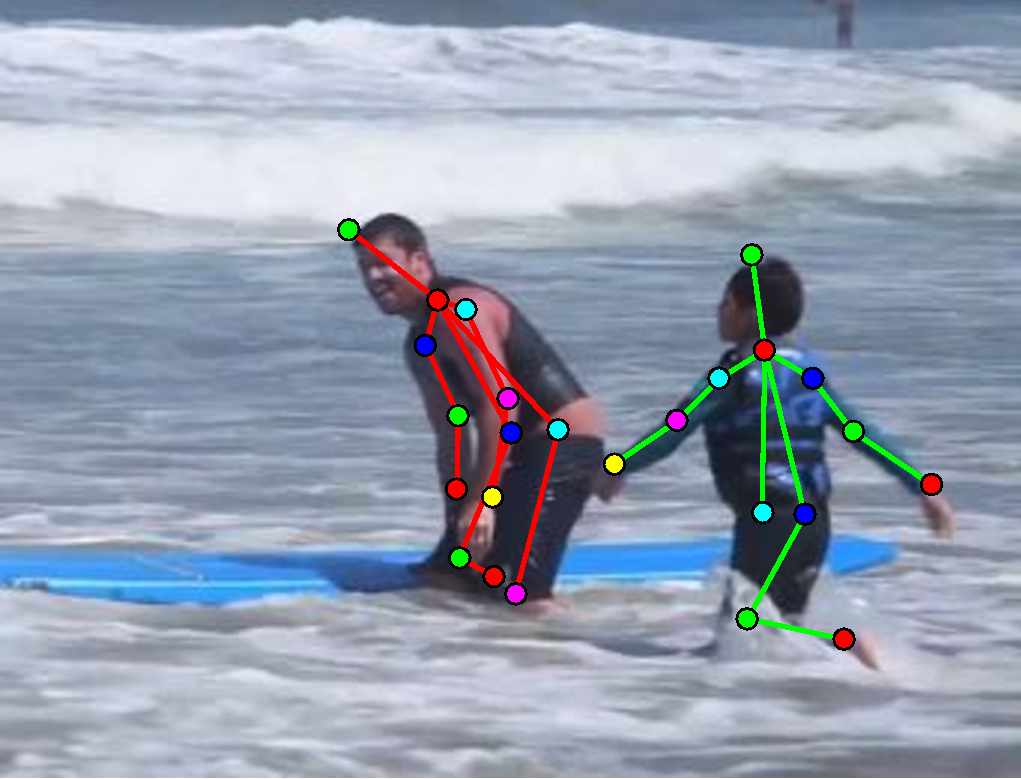
\includegraphics[height=0.140\linewidth]{imgidx_1183_sticks_mpii_multi.pdf}&
    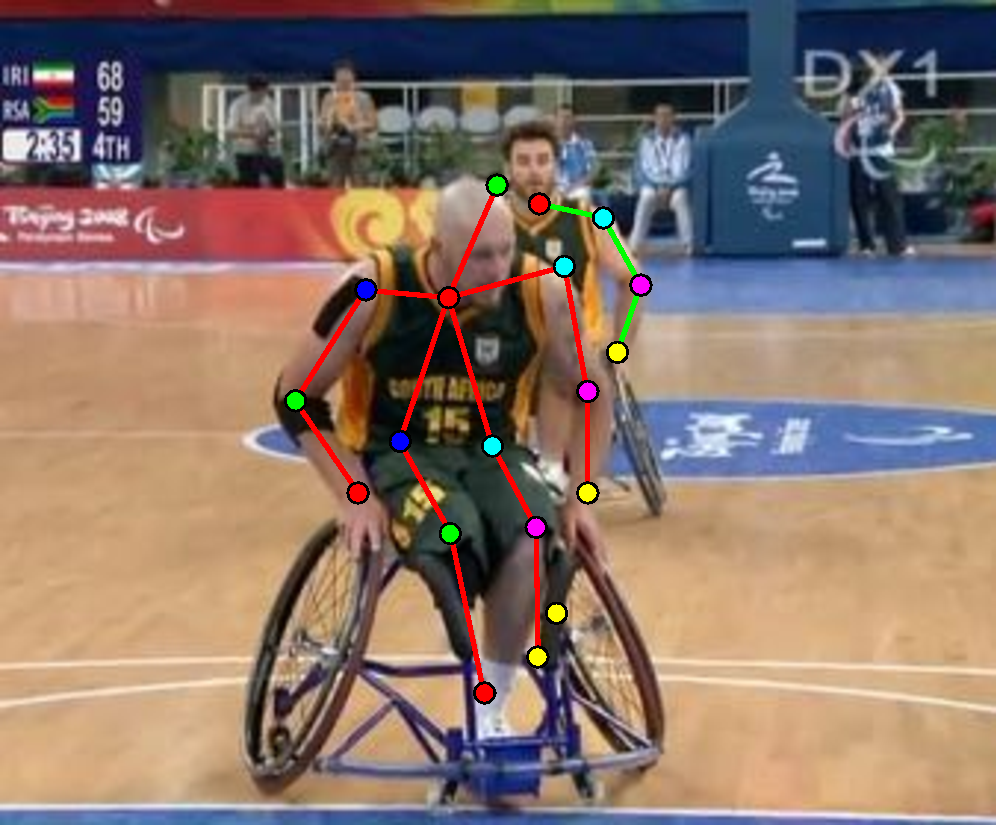
\includegraphics[height=0.140\linewidth]{imgidx_0094_sticks_mpii_multi.pdf}&
    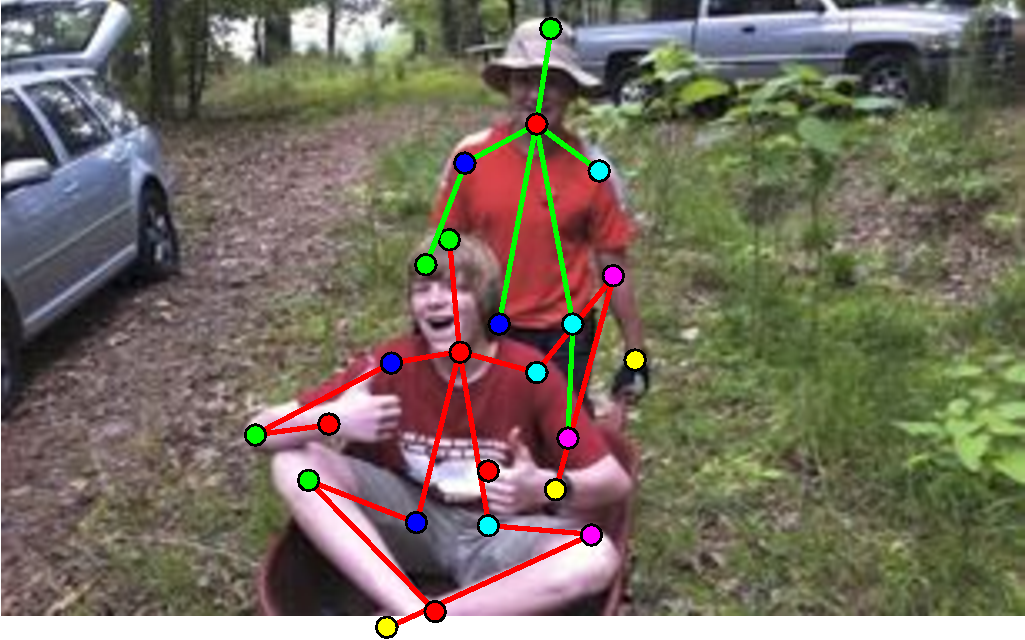
\includegraphics[height=0.140\linewidth]{imgidx_0903_sticks_mpii_multi.pdf}\\
    \midrule\midrule
    \begin{sideways}\bf \quad\quad$\detroi$\end{sideways}&

    \includegraphics[height=0.140\linewidth]{imgidx_0092_sticks_detroi_mpii_multi.pdf}&
    \includegraphics[height=0.140\linewidth]{imgidx_1366_sticks_detroi_mpii_multi.pdf}& 
%%     \includegraphics[height=0.140\linewidth]{imgidx_1589_sticks_detroi_mpii_multi.pdf}&
%%     \includegraphics[height=0.140\linewidth]{imgidx_1183_sticks_detroi_mpii_multi.pdf}&
    \includegraphics[height=0.140\linewidth]{imgidx_0094_sticks_detroi_mpii_multi.pdf}&
    \includegraphics[height=0.140\linewidth]{imgidx_0903_sticks_detroi_mpii_multi.pdf}\\
  &6&7&8&9\\  
  \end{tabular}
  %\vspace{-1em}
  \caption{Qualitative comparison of our joint formulation
    $\deepcut~\multb~\dense$ (rows 1-3, 5-7) to the traditional
    two-stage approach $\dense~\detroi$ (rows 4, 8) on MPII
    %Multi-Person dataset. 
    See Fig.~\ref{fig:overview} for the color-coding explanation.
    %See Fig.~\textcolor{red}{1} in paper for the color-coding explanation.
}
  \label{fig:qualitative_mpii}
\end{figure*}

\begin{figure*}
  \centering
  \begin{tabular}{c c c c c c c}
    &
    \includegraphics[height=0.140\linewidth]{imgidx_0075_init_graph_mpii_multi.pdf}&
    \includegraphics[height=0.140\linewidth]{imgidx_1017_init_graph_mpii_multi.pdf}&
    \includegraphics[height=0.140\linewidth]{imgidx_1033_init_graph_mpii_multi.pdf}&
    \includegraphics[height=0.140\linewidth]{imgidx_0210_init_graph_mpii_multi.pdf}&
    \includegraphics[height=0.140\linewidth]{imgidx_0697_init_graph_mpii_multi.pdf}\\
    \begin{sideways}\bf\quad $\deepcut~\multb$\end{sideways}&        
    \includegraphics[height=0.140\linewidth]{imgidx_0075_graph_mpii_multi.pdf}&
    \includegraphics[height=0.140\linewidth]{imgidx_1017_graph_mpii_multi.pdf}&
    \includegraphics[height=0.140\linewidth]{imgidx_1033_graph_mpii_multi.pdf}&
    \includegraphics[height=0.140\linewidth]{imgidx_0210_graph_mpii_multi.pdf}&
    \includegraphics[height=0.140\linewidth]{imgidx_0697_graph_mpii_multi.pdf}\\
    &
    \includegraphics[height=0.140\linewidth]{imgidx_0075_sticks_mpii_multi.pdf}&
    \includegraphics[height=0.140\linewidth]{imgidx_1017_sticks_mpii_multi.pdf}& 
    \includegraphics[height=0.140\linewidth]{imgidx_1033_sticks_mpii_multi.pdf}&
    \includegraphics[height=0.140\linewidth]{imgidx_0210_sticks_mpii_multi.pdf}&
    \includegraphics[height=0.140\linewidth]{imgidx_0697_sticks_mpii_multi.pdf}\\

    \midrule\midrule
    \begin{sideways}\bf \quad\quad$\detroi$\end{sideways}&
    \includegraphics[height=0.140\linewidth]{imgidx_0075_sticks_detroi_mpii_multi.pdf}&
    \includegraphics[height=0.140\linewidth]{imgidx_1017_sticks_detroi_mpii_multi.pdf}& 
    \includegraphics[height=0.140\linewidth]{imgidx_1033_sticks_detroi_mpii_multi.pdf}&
    \includegraphics[height=0.140\linewidth]{imgidx_0210_sticks_detroi_mpii_multi.pdf}&
    \includegraphics[height=0.140\linewidth]{imgidx_0697_sticks_detroi_mpii_multi.pdf}\\
    &10&11&12&13&14\\  
  \end{tabular}

  \begin{tabular}{c c c c c c c}
    \toprule
    &
    \includegraphics[height=0.140\linewidth]{imgidx_0908_init_graph_mpii_multi.pdf}&
    \includegraphics[height=0.140\linewidth]{imgidx_0104_init_graph_mpii_multi.pdf}&
    \includegraphics[height=0.140\linewidth]{imgidx_1589_init_graph_mpii_multi.pdf}&
    \includegraphics[height=0.140\linewidth]{imgidx_1183_init_graph_mpii_multi.pdf}&
    \includegraphics[height=0.140\linewidth]{imgidx_0568_init_graph_mpii_multi.pdf}&
    \includegraphics[height=0.140\linewidth]{imgidx_0804_init_graph_mpii_multi.pdf}\\
    \begin{sideways}\bf\quad $\deepcut~\multb$\end{sideways}&    
    \includegraphics[height=0.140\linewidth]{imgidx_0908_graph_mpii_multi.pdf}&
    \includegraphics[height=0.140\linewidth]{imgidx_0104_graph_mpii_multi.pdf}&
    \includegraphics[height=0.140\linewidth]{imgidx_1589_graph_mpii_multi.pdf}&
    \includegraphics[height=0.140\linewidth]{imgidx_1183_graph_mpii_multi.pdf}&
    \includegraphics[height=0.140\linewidth]{imgidx_0568_graph_mpii_multi.pdf}&
    \includegraphics[height=0.140\linewidth]{imgidx_0804_graph_mpii_multi.pdf}\\
    &
    \includegraphics[height=0.140\linewidth]{imgidx_0908_sticks_mpii_multi.pdf}&
    \includegraphics[height=0.140\linewidth]{imgidx_0104_sticks_mpii_multi.pdf}&
    \includegraphics[height=0.140\linewidth]{imgidx_1589_sticks_mpii_multi.pdf}&
    \includegraphics[height=0.140\linewidth]{imgidx_1183_sticks_mpii_multi.pdf}&
    \includegraphics[height=0.140\linewidth]{imgidx_0568_sticks_mpii_multi.pdf}&
    \includegraphics[height=0.140\linewidth]{imgidx_0804_sticks_mpii_multi.pdf}\\

    \midrule\midrule
    \begin{sideways}\bf \quad\quad$\detroi$\end{sideways}&
    \includegraphics[height=0.140\linewidth]{imgidx_0908_sticks_detroi_mpii_multi.pdf}&
    \includegraphics[height=0.140\linewidth]{imgidx_0104_sticks_detroi_mpii_multi.pdf}&
    \includegraphics[height=0.140\linewidth]{imgidx_1589_sticks_detroi_mpii_multi.pdf}&
    \includegraphics[height=0.140\linewidth]{imgidx_1183_sticks_detroi_mpii_multi.pdf}&
    \includegraphics[height=0.140\linewidth]{imgidx_0568_sticks_detroi_mpii_multi.pdf}&
    \includegraphics[height=0.140\linewidth]{imgidx_0804_sticks_detroi_mpii_multi.pdf}\\
    &15&16&17&18&19&20\\  
  \end{tabular}
  %\vspace{-1.0em}
  \caption{Qualitative comparison (contd.) of our joint formulation
    $\deepcut~\multb~\dense$ (rows 1-3, 5-7) to the traditional
    two-stage approach $\dense~\detroi$ (rows 4, 8) on MPII
    Multi-Person dataset. 
    See Fig.~\ref{fig:overview} for the color-coding explanation.
    %See Fig.~\textcolor{red}{1} in paper for the color-coding explanation.
    }
  \label{fig:qualitative_mpii2}
\end{figure*}

